% ============================================================
%  ANTOLOGÍA DE TÓPICOS DE MATEMÁTICAS
%  Universidad Autónoma de Nayarit
%  Licenciatura en Matemáticas
% ============================================================
\documentclass[12pt,letterpaper]{book}

\usepackage[utf8]{inputenc}
\usepackage[T1]{fontenc}
% babel no disponible para español en este entorno; se definen nombres manualmente

\usepackage{amsmath,amssymb,amsthm,mathtools}
\usepackage{cancel}

\usepackage{tikz}
\usetikzlibrary{arrows.meta,decorations.pathmorphing,patterns,
                calc,positioning,shapes.geometric,fit}
\usepackage{pgfplots}
\pgfplotsset{compat=1.18}

\usepackage[top=2.5cm,bottom=2.5cm,left=3cm,right=2.5cm,headheight=14pt]{geometry}
\usepackage{fancyhdr}
\usepackage{emptypage}

\usepackage[dvipsnames,svgnames,table]{xcolor}

% Paleta UAN
\definecolor{UANazul}  {RGB}{0,  68, 136}
\definecolor{UANoro}   {RGB}{204,153,  0}
\definecolor{UANgris}  {RGB}{ 96, 96, 96}
\definecolor{DefColor} {RGB}{230,240,255}
\definecolor{ThmColor} {RGB}{255,245,220}
\definecolor{PropColor}{RGB}{230,255,235}
\definecolor{EjColor}  {RGB}{245,245,245}
\definecolor{HistColor}{RGB}{240,230,250}
\definecolor{AplColor} {RGB}{255,237,213}
\definecolor{ActColor} {RGB}{222,247,222}

\usepackage[most]{tcolorbox}
\tcbuselibrary{breakable}

\newtcolorbox{defbox}[1]{enhanced, breakable, colback=DefColor, colframe=UANazul,
  fonttitle=\bfseries\color{white}, coltitle=white, colbacktitle=UANazul,
  title={#1}, arc=3pt, boxrule=0.7pt, left=6pt,right=6pt,top=4pt,bottom=4pt}

\newtcolorbox{thmbox}[1]{enhanced, breakable, colback=ThmColor, colframe=UANoro!80!black,
  fonttitle=\bfseries\color{white}, coltitle=white, colbacktitle=UANoro!80!black,
  title={#1}, arc=3pt, boxrule=0.7pt, left=6pt,right=6pt,top=4pt,bottom=4pt}

\newtcolorbox{propbox}[1]{enhanced, breakable, colback=PropColor, colframe=ForestGreen!60!black,
  fonttitle=\bfseries\color{white}, coltitle=white, colbacktitle=ForestGreen!60!black,
  title={#1}, arc=3pt, boxrule=0.7pt, left=6pt,right=6pt,top=4pt,bottom=4pt}

\newtcolorbox{ejbox}[1]{enhanced, breakable, colback=EjColor, colframe=UANgris,
  fonttitle=\bfseries\color{white}, coltitle=white, colbacktitle=UANgris,
  title={#1}, arc=3pt, boxrule=0.6pt, left=6pt,right=6pt,top=4pt,bottom=4pt}

\newtcolorbox{histbox}[1]{enhanced, breakable, colback=HistColor, colframe=Plum!70!black,
  fonttitle=\bfseries\color{white}, coltitle=white, colbacktitle=Plum!70!black,
  title={#1}, arc=3pt, boxrule=0.7pt, left=6pt,right=6pt,top=4pt,bottom=4pt}

\newtcolorbox{aplbox}[1]{enhanced, breakable, colback=AplColor, colframe=BurntOrange,
  fonttitle=\bfseries\color{white}, coltitle=white, colbacktitle=BurntOrange,
  title={#1}, arc=3pt, boxrule=0.7pt, left=6pt,right=6pt,top=4pt,bottom=4pt}

\newtcolorbox{actbox}[1]{enhanced, breakable, colback=ActColor, colframe=OliveGreen,
  fonttitle=\bfseries\color{white}, coltitle=white, colbacktitle=OliveGreen,
  title={#1}, arc=3pt, boxrule=0.7pt, left=6pt,right=6pt,top=4pt,bottom=4pt}

% Encabezados
\pagestyle{fancy}
\fancyhf{}
\renewcommand{\headrulewidth}{0.6pt}
\renewcommand{\footrulewidth}{0pt}
\fancyhead[LE,RO]{\small\color{UANazul}\thepage}
\fancyhead[RE]{\small\color{UANgris}\leftmark}
\fancyhead[LO]{\small\color{UANgris}\rightmark}

\usepackage{hyperref}
\hypersetup{colorlinks=true, linkcolor=UANazul, citecolor=UANazul, urlcolor=UANazul,
  pdftitle={Antología de Tópicos de Matemáticas}, pdfauthor={UAN}}

\usepackage{enumitem}
\setlist[enumerate,1]{label=\arabic*.}

\newcommand{\sen}{\operatorname{sen}}
\newcommand{\tg}{\operatorname{tg}}
\newcommand{\cotg}{\operatorname{cotg}}

\renewcommand{\chaptername}{Capítulo}
\renewcommand{\contentsname}{Índice general}
\renewcommand{\bibname}{Referencias}

\begin{document}

% ============================================================
\begin{titlepage}
\centering
\vspace*{1cm}
{\Large\bfseries\color{UANazul} Universidad Autónoma de Nayarit}\\[0.3cm]
{\large\color{UANgris} Licenciatura en Matemáticas}\\[2cm]


\begin{tikzpicture}
\draw[UANazul, line width=1pt] (-6,0) -- (6,0);
\end{tikzpicture}

\vspace{1cm}
{\huge\bfseries\color{UANazul} Antología de Tópicos\\[0.2cm] de Matemáticas}\\[1.5cm]

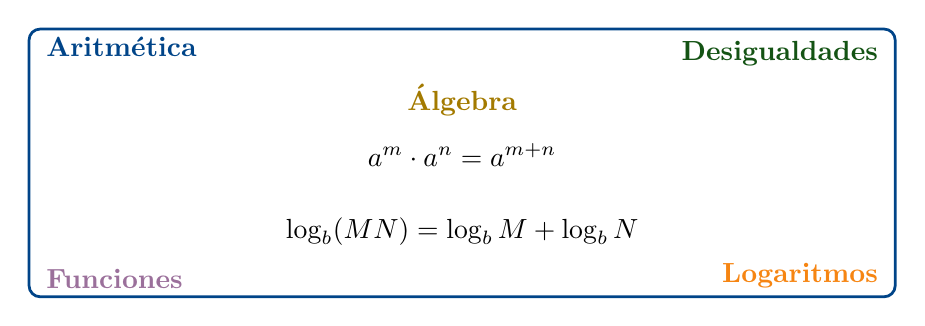
\begin{tikzpicture}[scale=1]
\node[draw=UANazul, line width=1pt, rounded corners, minimum width=11cm, minimum height=3.4cm] (box) at (0,0) {};
\node[anchor=north west, font=\bfseries\color{UANazul}] at (box.north west) {\;Aritmética};
\node[anchor=north] at ([yshift=-0.6cm]box.north) {\bfseries\color{UANoro!80!black} Álgebra};
\node[anchor=north east, font=\bfseries\color{ForestGreen!60!black}] at ([yshift=-0.05cm]box.north east) {Desigualdades\;};
\node[anchor=center] at ([yshift=0.1cm]box.center) {$\displaystyle a^m\cdot a^n = a^{m+n}$};
\node[anchor=south west, font=\bfseries\color{Plum!70!black}] at (box.south west) {\;Funciones};
\node[anchor=south east, font=\bfseries\color{BurntOrange}] at (box.south east) {Logaritmos\;};
\node[anchor=south] at ([yshift=0.55cm]box.south) {$\displaystyle \log_b(MN)=\log_b M + \log_b N$};
\end{tikzpicture}

\vfill
{\large\color{UANgris} Tepic, Nayarit -- 2026}
\end{titlepage}

\cleardoublepage

% ============================================================
\tableofcontents
\cleardoublepage

% ============================================================
\chapter{Aritmética elemental}

\section*{Antecedentes: Los conjuntos numéricos}
\addcontentsline{toc}{section}{Antecedentes: Los conjuntos numéricos}

Antes de operar con números es indispensable conocer los conjuntos a los que pertenecen.
Los números reales se organizan en una jerarquía de conjuntos anidados que pasamos a ilustrar.

\begin{center}
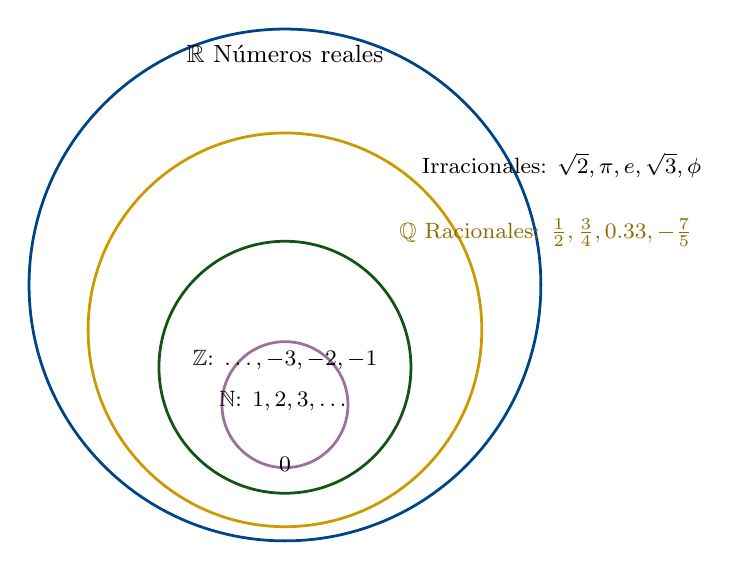
\begin{tikzpicture}[scale=0.95]
\node[draw, circle, minimum size=6.5cm, UANazul, line width=1pt] (R) at (0,0) {};
\node[draw, circle, minimum size=5cm, UANoro, line width=1pt] (Q) at (0,-0.6) {};
\node[draw, circle, minimum size=3.2cm, ForestGreen!60!black, line width=1pt] (Z) at (0,-1.1) {};
\node[draw, circle, minimum size=1.6cm, Plum!70!black, line width=1pt] (N) at (0,-1.6) {};
\node[anchor=north, yshift=-0.1cm] at (R.north) {\small $\mathbb{R}$ Números reales};
\node[anchor=west] at (1.7,1.6) {\footnotesize Irracionales: $\sqrt{2},\pi,e,\sqrt{3},\phi$};
\node[anchor=west,UANoro!70!black] at (1.4,0.7) {\footnotesize $\mathbb{Q}$ Racionales: $\tfrac12,\tfrac34,0.33,-\tfrac75$};
\node at (0,-1.0) {\footnotesize $\mathbb{Z}$: $\dots,-3,-2,-1$};
\node at (0,-1.55) {\footnotesize $\mathbb{N}$: $1,2,3,\dots$};
\node at (0,-2.4) {\footnotesize $0$};
\end{tikzpicture}

\vspace{0.3cm}
$\mathbb{N}\subset\mathbb{Z}\subset\mathbb{Q}\subset\mathbb{R}$

\vspace{0.3cm}
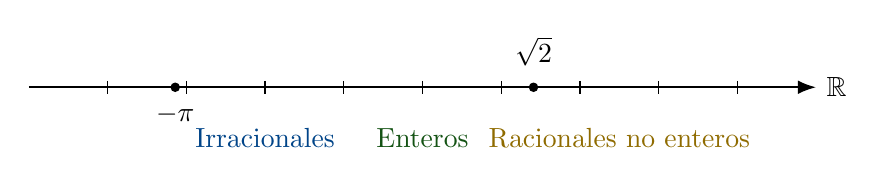
\begin{tikzpicture}
\draw[line width=0.8pt,-{Latex}] (-5,0) -- (5,0) node[right] {$\mathbb{R}$};
\foreach \x in {-4,-3,-2,-1,0,1,2,3,4} \draw (\x,0.08) -- (\x,-0.08);
\node[below] at (-3.14,-0.1) {$-\pi$};
\node[below] at (-1.41,-0.1) {};
\filldraw (-3.14,0) circle (1.5pt);
\filldraw (1.41,0) circle (1.5pt);
\node[above] at (1.41,0.15) {$\sqrt2$};
\node[below,UANazul] at (-2,-0.4) {Irracionales};
\node[below,ForestGreen!60!black] at (0,-0.4) {Enteros};
\node[below,UANoro!70!black] at (2.5,-0.4) {Racionales no enteros};
\end{tikzpicture}
\end{center}

\textbf{Objetivo del capítulo.} El estudiante aplicará las operaciones fundamentales sobre los
números reales, interpretará el valor absoluto, manejará exponentes y radicales, y resolverá
razones y proporciones.

\section{Operaciones elementales}

\begin{defbox}{Definición 1.1. Operaciones elementales}
Sean $a,b\in\mathbb{R}$. Las cuatro operaciones elementales son:
\[ a+b\ (\text{suma}),\quad a-b\ (\text{diferencia}),\quad a\cdot b\ (\text{producto}),\quad \frac{a}{b}\ (b\neq0)\ (\text{cociente}). \]
\end{defbox}

\begin{defbox}{Definición 1.2. Jerarquía de operaciones}
\begin{enumerate}
\item Paréntesis, corchetes y llaves.
\item Potencias y raíces.
\item Multiplicación y división (izquierda a derecha).
\item Adición y sustracción (izquierda a derecha).
\end{enumerate}
\end{defbox}

\begin{propbox}{Propiedad 1.1. Propiedades de los números reales}
Para todo $a,b,c\in\mathbb{R}$:\\
\textbf{Conmutatividad:} $a+b=b+a$, $ab=ba$.\\
\textbf{Asociatividad:} $(a+b)+c=a+(b+c)$, $(ab)c=a(bc)$.\\
\textbf{Distributividad:} $a(b+c)=ab+ac$.\\
\textbf{Neutros:} $a+0=a$, $a\cdot1=a$.\\
\textbf{Inversos:} $a+(-a)=0$, $a\cdot\frac{1}{a}=1$ ($a\neq0$).
\end{propbox}

\begin{ejbox}{Ejemplo 1.1. Jerarquía básica}
Evalúa $8+3\times2-(4+1)$. \textit{Solución:} $8+6-5=9$.
\end{ejbox}

\begin{ejbox}{Ejemplo 1.2. Expresión fraccionaria}
Evalúa $\dfrac{3\times(4+2)^2-6}{3}$. \textit{Solución:} $\dfrac{102}{3}=34$.
\end{ejbox}

\begin{ejbox}{Ejemplo 1.3. Corchetes anidados}
Simplifica $2[3+(5-1)\cdot2]-\dfrac{4^3}{2^2-5}$. \textit{Solución:} $\dfrac{18}{4}=\dfrac{9}{2}$.
\end{ejbox}

\section{Valor absoluto de números reales}

\begin{defbox}{Definición 1.3. Valor absoluto}
\[ |a| = \begin{cases} a & a\geq0\\ -a & a<0 \end{cases} \]
Geométricamente: distancia de $a$ al origen en $\mathbb{R}$.
\end{defbox}

\begin{center}
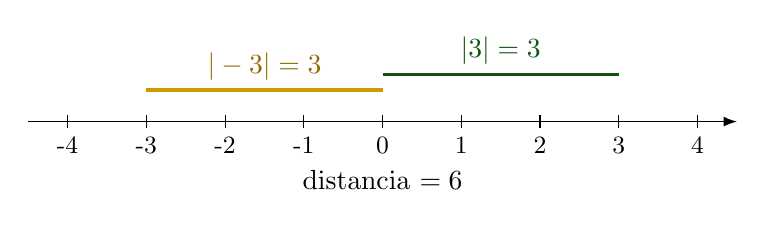
\begin{tikzpicture}
\draw[-{Latex}] (-4.5,0) -- (4.5,0);
\foreach \x in {-4,-3,-2,-1,0,1,2,3,4} \draw (\x,0.08)--(\x,-0.08) node[below]{\small\x};
\draw[UANoro,line width=1.2pt] (-3,0.4) -- (0,0.4);
\draw[ForestGreen!60!black,line width=1.2pt] (0,0.6) -- (3,0.6);
\node[above,UANoro!70!black] at (-1.5,0.4) {$|-3|=3$};
\node[above,ForestGreen!60!black] at (1.5,0.6) {$|3|=3$};
\node[below] at (0,-0.5) {distancia $=6$};
\end{tikzpicture}
\end{center}

\begin{propbox}{Propiedad 1.2. Propiedades del valor absoluto}
$|a|\geq0$;\quad $|a|=0\Leftrightarrow a=0$;\quad $|ab|=|a||b|$;\quad $|a/b|=|a|/|b|$;\quad $|-a|=|a|$.
\end{propbox}

\begin{thmbox}{Teorema 1.1. Desigualdad triangular}
$|a+b|\leq|a|+|b|$ para todo $a,b\in\mathbb{R}$.\\[2pt]
\textit{Dem.} Como $-|a|\leq a\leq|a|$ y $-|b|\leq b\leq|b|$, sumando: $-(|a|+|b|)\leq a+b\leq|a|+|b|$, lo que equivale a la tesis. $\square$
\end{thmbox}

\begin{ejbox}{Ejemplo 1.4. Cálculo directo}
$|-7|=7$;\quad $|4.5|=4.5$;\quad $|0|=0$.
\end{ejbox}

\begin{ejbox}{Ejemplo 1.5. Combinación}
$|3-8|+|-2\cdot5| = 5+10 = 15$.
\end{ejbox}

\begin{ejbox}{Ejemplo 1.6. Ecuación con valor absoluto}
Resuelve $|2x-4|=6$. \textit{Solución:} $2x-4=6\Rightarrow x=5$; $2x-4=-6\Rightarrow x=-1$. $x\in\{-1,5\}$.
\end{ejbox}

\section{Exponentes}
\subsection{Exponentes enteros}

\begin{defbox}{Definición 1.4. Potencia}
$a^n = \underbrace{a\cdots a}_{n}$;\quad $a^0=1$;\quad $a^{-n}=1/a^n$ ($a\neq0$).
\end{defbox}

\subsection{Leyes de exponentes}

\begin{propbox}{Propiedad 1.3. Leyes de los exponentes}
Para $a,b\neq0$, $m,n\in\mathbb{Z}$:
\begin{center}
\begin{tabular}{lll}
\textbf{Ley} & \textbf{Fórmula} & \textbf{Ejemplo}\\\hline
Producto & $a^m\cdot a^n=a^{m+n}$ & $2^3\cdot2^4=2^7=128$\\
Cociente & $a^m/a^n=a^{m-n}$ & $3^5/3^2=3^3=27$\\
Potencia de potencia & $(a^m)^n=a^{mn}$ & $(5^2)^3=5^6$\\
Potencia de producto & $(ab)^n=a^nb^n$ & $(2x)^3=8x^3$\\
Potencia de cociente & $(a/b)^n=a^n/b^n$ & $(x/3)^2=x^2/9$\\
Exponente negativo & $a^{-n}=1/a^n$ & $5^{-2}=1/25$
\end{tabular}
\end{center}
\end{propbox}

\begin{thmbox}{Teorema 1.2. Demostración de las leyes de exponentes}
\textbf{(1) Ley del producto.} Para $m,n\in\mathbb{N}$: $a^m\cdot a^n=(\underbrace{a\cdots a}_m)(\underbrace{a\cdots a}_n)=\underbrace{a\cdots a}_{m+n}=a^{m+n}$. $\square$\\[4pt]
\textbf{(2) Ley del cociente} ($a\neq0,\,m>n$): $a^m/a^n=a^{m-n}$, cancelando $n$ factores comunes. $\square$\\[4pt]
\textbf{(3) Potencia de potencia:} $(a^m)^n=\underbrace{a^m\cdots a^m}_{n}=a^{m+\cdots+m}=a^{mn}$. $\square$\\[4pt]
\textbf{(4) Exponente cero:} por la ley del cociente con $m=n$: $a^0=a^{n-n}=a^n/a^n=1$ ($a\neq0$). $\square$\\[4pt]
\textbf{(5) Exponente negativo:} $a^{-n}=a^{0-n}=a^0/a^n=1/a^n$. $\square$
\end{thmbox}

\begin{ejbox}{Ejemplo 1.7. Ley del producto}
$3^4\cdot3^{-2}=3^{4-2}=3^2=9$.
\end{ejbox}

\begin{ejbox}{Ejemplo 1.8. Combinación de leyes}
$\dfrac{(2^3)^2\cdot2^{-4}}{2^2}=\dfrac{2^6\cdot2^{-4}}{2^2}=\dfrac{2^2}{2^2}=1$.
\end{ejbox}

\begin{ejbox}{Ejemplo 1.9. Expresión con variables}
$\dfrac{x^3y^{-2}(xy)^2}{x^{-1}y^3}=\dfrac{x^5y^0}{x^{-1}y^3}=x^6y^{-3}=\dfrac{x^6}{y^3}$.
\end{ejbox}

\subsection{Exponentes racionales}

\begin{defbox}{Definición 1.5. Exponente racional}
$a^{m/n}=\sqrt[n]{a^m}=(\sqrt[n]{a})^m$ ($a>0$, $n\geq2$).
\end{defbox}

\begin{ejbox}{Ejemplo 1.10. Evaluación}
$8^{2/3}=(\sqrt[3]{8})^2=2^2=4$.
\end{ejbox}

\begin{ejbox}{Ejemplo 1.11. Simplificación}
$\dfrac{x^{3/2}\cdot x^{1/2}}{x^{1/3}}=x^{2-1/3}=x^{5/3}$.
\end{ejbox}

\section{Radicales}

\begin{defbox}{Definición 1.6. Radical}
$\sqrt[n]{a}=a^{1/n}$ es el número no negativo $b$ tal que $b^n=a$. $n$: índice; $a$: radicando.
\end{defbox}

\begin{propbox}{Propiedad 1.4. Propiedades de los radicales}
$\sqrt[n]{a}\cdot\sqrt[n]{b}=\sqrt[n]{ab}$;\quad $\sqrt[n]{a}/\sqrt[n]{b}=\sqrt[n]{a/b}$;\quad $(\sqrt[n]{a})^m=a^{m/n}$;\quad $\sqrt[m]{\sqrt[n]{a}}=\sqrt[mn]{a}$.
\end{propbox}

\subsection{Simplificación}

\begin{defbox}{Definición 1.7. Radical simplificado}
$\sqrt[n]{a}$ está simplificado si el radicando no tiene factores que sean potencias $n$-ésimas perfectas.
\end{defbox}

\begin{ejbox}{Ejemplo 1.12. Raíz cuadrada}
$\sqrt{48}=\sqrt{16\cdot3}=4\sqrt3$.
\end{ejbox}

\begin{ejbox}{Ejemplo 1.13. Raíz cúbica con variables}
$\sqrt[3]{54x^4y^5}=3xy\sqrt[3]{2xy^2}$.
\end{ejbox}

\begin{ejbox}{Ejemplo 1.14. Suma de radicales}
$3\sqrt{12}-2\sqrt{27}+\sqrt{75}=(6-6+5)\sqrt3=5\sqrt3$.
\end{ejbox}

\subsection{Racionalización}

\begin{defbox}{Definición 1.8. Racionalización}
Eliminar radicales del denominador multiplicando por una expresión conveniente.
\end{defbox}

\begin{propbox}{Propiedad 1.5. Conjugado binomial}
$(\sqrt a+\sqrt b)(\sqrt a-\sqrt b)=a-b$.
\end{propbox}

\begin{ejbox}{Ejemplo 1.15. Racionalización simple}
$\dfrac{3}{\sqrt5}\cdot\dfrac{\sqrt5}{\sqrt5}=\dfrac{3\sqrt5}{5}$.
\end{ejbox}

\begin{ejbox}{Ejemplo 1.16. Racionalización con conjugado}
$\dfrac{4}{1+\sqrt3}\cdot\dfrac{1-\sqrt3}{1-\sqrt3}=\dfrac{4(1-\sqrt3)}{-2}=2\sqrt3-2$.
\end{ejbox}

\begin{ejbox}{Ejemplo 1.17. Dos radicales en el denominador}
Racionaliza $\dfrac{6}{\sqrt5+\sqrt2}$. \textit{Solución:} $\dfrac{6(\sqrt5-\sqrt2)}{3}=2(\sqrt5-\sqrt2)$.
\end{ejbox}

\begin{ejbox}{Ejemplo 1.18. Racionalización con índice 3}
Racionaliza $\dfrac{2}{\sqrt[3]4}$. \textit{Solución:} $\dfrac{2\sqrt[3]2}{2}=\sqrt[3]2$.
\end{ejbox}

\begin{ejbox}{Ejemplo 1.19. Racionalización doble}
Simplifica $\dfrac{\sqrt x-\sqrt y}{\sqrt x+\sqrt y}=\dfrac{x-2\sqrt{xy}+y}{x-y}$.
\end{ejbox}

\begin{ejbox}{Ejemplo 1.20. Racionalización con parámetro}
Racionaliza $\dfrac{\sqrt{a+h}-\sqrt a}{h}$ ($h\neq0$). \textit{Solución:} $\dfrac{1}{\sqrt{a+h}+\sqrt a}$. (Aparece al calcular la derivada de $\sqrt x$.)
\end{ejbox}

\section{Razones y proporciones}

\begin{defbox}{Definición 1.9. Razón, proporción y tipos de proporcionalidad}
La razón de $a$ a $b$ ($b\neq0$) es $a/b$. Cuatro números forman una proporción si $a/b=c/d\Leftrightarrow ad=bc$.\\
\textbf{Proporción directa:} $y=kx$ ($k>0$). \textbf{Proporción inversa:} $y=k/x$ ($k>0$).
\end{defbox}

\begin{center}
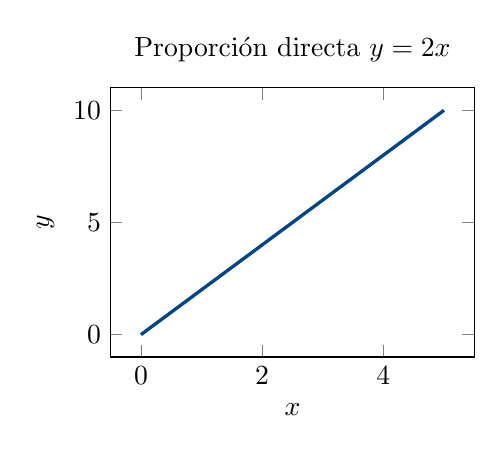
\begin{tikzpicture}
\begin{axis}[width=6.2cm,height=5cm,xlabel=$x$,ylabel=$y$,title={Proporción directa $y=2x$}]
\addplot[UANazul,line width=1.2pt,domain=0:5] {2*x};
\end{axis}
\end{tikzpicture}
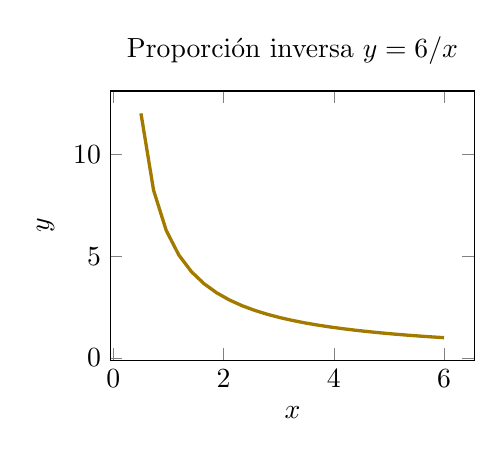
\begin{tikzpicture}
\begin{axis}[width=6.2cm,height=5cm,xlabel=$x$,ylabel=$y$,title={Proporción inversa $y=6/x$}]
\addplot[UANoro!80!black,line width=1.2pt,domain=0.5:6] {6/x};
\end{axis}
\end{tikzpicture}
\end{center}

\begin{propbox}{Teorema 1.3. Propiedades de las proporciones}
Si $a/b=c/d$: (1) $ad=bc$ (productos cruzados). (2) $a/c=b/d$ (alternando). (3) $(a+b)/b=(c+d)/d$ (componendo). (4) $(a-b)/b=(c-d)/d$ (dividendo).
\end{propbox}

\begin{ejbox}{Ejemplo 1.21. Proporción simple}
Si $x/12=5/8$, encuentra $x$. \textit{Solución:} $x=60/8=7.5$.
\end{ejbox}

\begin{ejbox}{Ejemplo 1.22. Proporción aplicada -- mapa}
2 cm representan 50 km. ¿Cuántos km son 7 cm? \textit{Solución:} $2/50=7/x\Rightarrow x=175$ km.
\end{ejbox}

\begin{ejbox}{Ejemplo 1.23. Razón compuesta}
Edades en razón $2:3:5$ y suman 60. \textit{Solución:} $k=6$; edades: 12, 18, 30 años.
\end{ejbox}

\begin{ejbox}{Ejemplo 1.24. Proporción directa}
El costo de gasolina es directamente proporcional a los litros comprados. Si 10 L cuestan \$230, ¿cuánto cuestan 35 L? \textit{Solución:} $k=23$ \$/L. $C=23\cdot35=\$805$.
\end{ejbox}

\begin{ejbox}{Ejemplo 1.25. Proporción inversa}
Un automóvil tarda 3 h a 80 km/h. ¿Cuánto tarda a 120 km/h? \textit{Solución:} $k=240$. Tiempo $=240/120=2$ h.
\end{ejbox}

\begin{ejbox}{Ejemplo 1.26. Regla de tres compuesta}
6 obreros pintan un muro en 4 días trabajando 8 h/día. ¿Cuántos días tardan 4 obreros trabajando 6 h/día? \textit{Solución:} $192/(4\times6)=8$ días.
\end{ejbox}

\begin{aplbox}{Problema de aplicación 1.1. Mezclas}
Una solución de ácido al 30\% se mezcla con otra al 60\% para obtener 10 litros de una solución al 45\%. ¿Cuántos litros de cada una se requieren?\\
\textit{Solución:} Sea $x$ los litros al 30\%. $0.30x+0.60(10-x)=0.45(10)\Rightarrow x=5$ litros de cada una.
\end{aplbox}

\begin{aplbox}{Problema de aplicación 1.2. Escalas}
Un plano arquitectónico usa una escala de $1:150$. Si una habitación mide 3.2 cm en el plano, ¿cuál es su longitud real?\\
\textit{Solución:} $3.2\times150=480$ cm $=4.8$ m.
\end{aplbox}

\section{Ejercicios propuestos}

\begin{enumerate}
\item Evalúa: $5+3\times(8-2)\div9$.
\item Simplifica: $2[4+3(5-2)]-10$.
\item Calcula: $\dfrac{4^2-2\times3}{(3+1)^2-5}$.
\item Evalúa: $|-9|-|4-7|+|0|$.
\item Resuelve: $|3x+1|=10$.
\item Verifica la desigualdad triangular con $a=-4$, $b=7$.
\item Simplifica: $x^5\cdot x^{-3}\cdot x^0$.
\item Calcula: $\left(\dfrac{2^3\cdot2^{-1}}{2^4}\right)^2$.
\item Expresa como radical: $a^{3/4}$.
\item Simplifica: $\dfrac{a^{2/3}\cdot a^{1/2}}{a^{1/6}}$.
\item Simplifica: $\sqrt{200}$.
\item Opera: $2\sqrt8+3\sqrt{18}-\sqrt{50}$.
\item Racionaliza: $\dfrac{6}{\sqrt7-1}$.
\item Racionaliza: $\dfrac{3}{\sqrt[3]9}$.
\item Simplifica: $\sqrt[3]{16a^5b^7}$.
\item Resuelve la proporción: $\dfrac{x+1}{5}=\dfrac{x-2}{3}$.
\item Los lados de un triángulo están en razón $3:4:5$ y el perímetro es 72 cm.
\item Si 4 obreros terminan una obra en 15 días, ¿cuántos días tardan 6 obreros?
\item El precio de un artículo es directamente proporcional a su peso. Si 3 kg cuestan \$120, ¿cuánto cuestan 7.5 kg?
\item Un depósito se llena con 5 tuberías en 6 horas. ¿Cuántas horas tarda con 3 tuberías?
\item \textit{(Nuevo)} Evalúa: $\dfrac{(-2)^3-3(-2)^2+5}{|-7|-2}$.
\item \textit{(Nuevo)} Simplifica: $\sqrt[4]{81x^8y^{12}}$.
\item \textit{(Nuevo)} Racionaliza el denominador: $\dfrac{5}{2-\sqrt3}$.
\item \textit{(Nuevo)} Resuelve: $\left|\dfrac{2x-1}{3}\right|=5$.
\item \textit{(Nuevo)} Demuestra que $\sqrt{a^2}=|a|$ para todo $a\in\mathbb{R}$ usando la definición de valor absoluto.
\item \textbf{(Aplicación)} Una receta para 8 personas requiere 350 g de harina. ¿Cuánta harina se necesita para 20 personas?
\item \textbf{(Aplicación)} Un capital de \$15{,}000 se reparte entre tres socios en razón $2:3:5$ según su inversión. ¿Cuánto recibe cada uno?
\item \textbf{(Aplicación)} La intensidad luminosa de una fuente puntual es inversamente proporcional al cuadrado de la distancia. Si a 2 m la intensidad es 80 lux, ¿cuál es la intensidad a 5 m?
\item \textbf{(Aplicación)} Un tinaco se llena con una llave en 5 horas y se vacía con una fuga en 8 horas. Si ambas están abiertas, ¿en cuánto tiempo se llena?
\item \textbf{(Aplicación)} Para fabricar 120 piezas, una máquina tarda 9 horas. ¿Cuántas piezas fabrica en una jornada de 6 horas trabajando al mismo ritmo?
\end{enumerate}

\textbf{Respuestas (1--20):} 1. $7$\quad 2. $16$\quad 3. $5/6$\quad 4. $6$\quad 5. $x=3$ ó $-11/3$\quad 6. $3\leq11$ \checkmark\quad 7. $x^2$\quad 8. $1/4$\quad 9. $\sqrt[4]{a^3}$\quad 10. $a$\quad 11. $10\sqrt2$\quad 12. $10\sqrt2$\quad 13. $\sqrt7+1$\quad 14. $\sqrt[3]{3}/3$\quad 15. $2ab^2\sqrt[3]{2a^2b}$\quad 16. $x=13/2$\quad 17. $18,24,30$ cm\quad 18. $10$ días\quad 19. \$300\quad 20. $10$ h.

\textbf{Respuestas (21--30):} 21. $4$\quad 22. $3xy^2\sqrt[4]{x^4y^0}=3x^2y^3$\quad 23. $5(2+\sqrt3)$\quad 24. $x=8$ ó $x=-7$\quad 25. Se sigue de $\sqrt{a^2}=|a|\geq0$ y $|a|^2=a^2$\quad 26. $875$ g\quad 27. \$3{,}000, \$4{,}500, \$7{,}500\quad 28. $12.8$ lux\quad 29. $\approx6.15$ h\quad 30. $80$ piezas.

% ============================================================
\chapter{Elementos de álgebra}

\section*{Antecedentes: El paso de la aritmética al álgebra}
\addcontentsline{toc}{section}{Antecedentes: El paso de la aritmética al álgebra}

El álgebra introduce variables que representan números desconocidos. La siguiente
ilustración muestra cómo una misma situación pasa del lenguaje aritmético al algebraico.

\begin{center}
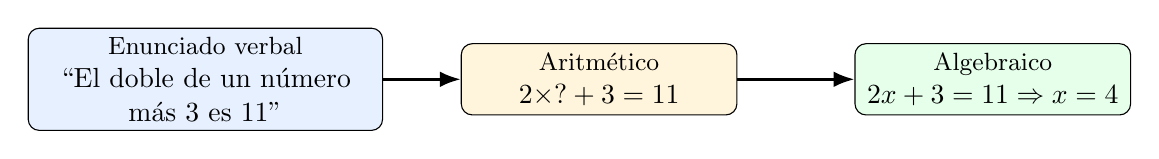
\begin{tikzpicture}
\node[draw,rounded corners,fill=DefColor,align=center,minimum width=4.5cm] (v) at (0,0) {\small Enunciado verbal\\``El doble de un número\\más 3 es 11''};
\node[draw,rounded corners,fill=ThmColor,align=center,minimum width=3.5cm] (a) at (5,0) {\small Aritmético\\$2\times?+3=11$};
\node[draw,rounded corners,fill=PropColor,align=center,minimum width=3.5cm] (b) at (10,0) {\small Algebraico\\$2x+3=11\Rightarrow x=4$};
\draw[-{Latex},line width=1pt] (v) -- (a);
\draw[-{Latex},line width=1pt] (a) -- (b);
\end{tikzpicture}
\end{center}

\textbf{Objetivo del capítulo.} Utilizar el lenguaje algebraico para expresar relaciones, operar con polinomios, factorizar y resolver ecuaciones.

\section{Lenguaje algebraico}

\begin{defbox}{Definición 2.1. Expresión algebraica}
Combinación de variables, coeficientes y operaciones. Sus elementos: variable, coeficiente, exponente, término, término independiente.\\[4pt]
\centering $\underbrace{3}_{\text{coef.}}x^{\overbrace{2}^{\text{exp.}}} - 5xy + \underbrace{7}_{\text{término indep.}}$
\end{defbox}

\begin{ejbox}{Ejemplo 2.1. Términos semejantes}
$3x^2+2x^2-5xy+y = 5x^2-5xy+y$.
\end{ejbox}

\section{Operaciones algebraicas fundamentales}

\begin{ejbox}{Ejemplo 2.2. Suma de polinomios}
$(2x^3-3x+4)+(-x^3+5x-1)=x^3+2x+3$.
\end{ejbox}

\begin{ejbox}{Ejemplo 2.3. Multiplicación de polinomios}
$(2x-1)(x^2+3x-2)=2x^3+5x^2-7x+2$.
\end{ejbox}

\section{Productos notables}

\begin{propbox}{Propiedad 2.1. Productos notables fundamentales}
\begin{align}
(a+b)^2 &= a^2+2ab+b^2\\
(a-b)^2 &= a^2-2ab+b^2\\
(a+b)(a-b) &= a^2-b^2\\
(a+b)^3 &= a^3+3a^2b+3ab^2+b^3\\
(a-b)^3 &= a^3-3a^2b+3ab^2-b^3
\end{align}
\end{propbox}

\begin{thmbox}{Teorema 2.1. Demostración geométrica de $(a+b)^2=a^2+2ab+b^2$}
\begin{center}
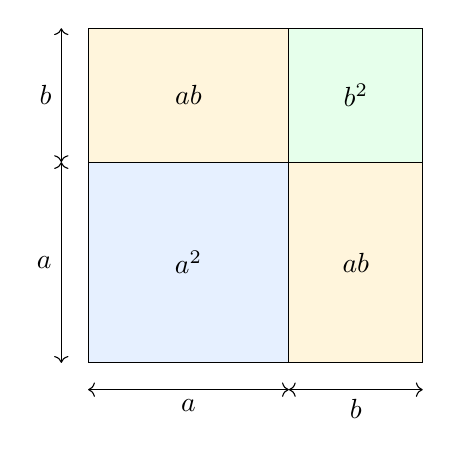
\begin{tikzpicture}[scale=0.85]
\draw[fill=DefColor] (0,0) rectangle (3,3);
\draw[fill=ThmColor] (3,0) rectangle (5,3);
\draw[fill=ThmColor] (0,3) rectangle (3,5);
\draw[fill=PropColor] (3,3) rectangle (5,5);
\node at (1.5,1.5) {$a^2$};
\node at (4,1.5) {$ab$};
\node at (1.5,4) {$ab$};
\node at (4,4) {$b^2$};
\draw[<->] (0,-0.4) -- (3,-0.4) node[midway,below]{$a$};
\draw[<->] (3,-0.4) -- (5,-0.4) node[midway,below]{$b$};
\draw[<->] (-0.4,0) -- (-0.4,3) node[midway,left]{$a$};
\draw[<->] (-0.4,3) -- (-0.4,5) node[midway,left]{$b$};
\end{tikzpicture}
\end{center}
El cuadrado de lado $(a+b)$ se descompone en cuatro regiones. Área total $=(a+b)^2=a^2+ab+ab+b^2=a^2+2ab+b^2$. $\square$
\end{thmbox}

\begin{thmbox}{Teorema 2.2. Demostración geométrica de $a^2-b^2=(a+b)(a-b)$}
Recortando un cuadrado de lado $b$ de la esquina de un cuadrado de lado $a$ y reagrupando las piezas restantes se forma un rectángulo de lados $(a+b)$ y $(a-b)$, cuya área es $a^2-b^2$. $\square$
\end{thmbox}

\begin{ejbox}{Ejemplo 2.4. Cuadrado de binomio}
$(3x-2)^2=9x^2-12x+4$.
\end{ejbox}

\begin{ejbox}{Ejemplo 2.5. Diferencia de cuadrados}
$(5x+3)(5x-3)=25x^2-9$.
\end{ejbox}

\begin{ejbox}{Ejemplo 2.6. Cubo de binomio}
$(x+2)^3=x^3+6x^2+12x+8$.
\end{ejbox}

\begin{aplbox}{Problemas con productos notables}
\textbf{a)} Calcula mentalmente $98^2$ usando $(100-2)^2$.\\
\textit{Solución:} $(100-2)^2=10000-400+4=9604$.\\[4pt]
\textbf{b)} Calcula $61\times59$ usando diferencia de cuadrados.\\
\textit{Solución:} $61\times59=(60+1)(60-1)=3600-1=3599$.\\[4pt]
\textbf{c)} El área de un cuadrado de lado $(x+5)$ representa el área de un terreno cuadrado. Exprésala como trinomio y evalúa para $x=12$ m.\\
\textit{Solución:} $(x+5)^2=x^2+10x+25$; para $x=12$: $144+120+25=289$ m$^2$.\\[4pt]
\textbf{d)} Un cubo de arista $(a-3)$ cm representa el volumen restante tras tallar un cubo menor. Expresa su volumen desarrollado y evalúa para $a=10$.\\
\textit{Solución:} $(a-3)^3=a^3-9a^2+27a-27$; para $a=10$: $1000-900+270-27=343$ cm$^3$.\\[4pt]
\textbf{e)} Simplifica usando productos notables: $\dfrac{(x+3)^2-(x-3)^2}{4x}$.\\
\textit{Solución:} El numerador es una diferencia de cuadrados de binomios: $[(x+3)+(x-3)][(x+3)-(x-3)]=2x\cdot6=12x$. El resultado es $\dfrac{12x}{4x}=3$.
\end{aplbox}

\subsection{Binomio de Newton y Triángulo de Pascal}

\begin{thmbox}{Teorema 2.3. Binomio de Newton}
Para $n\in\mathbb{N}$:
\[ (a+b)^n=\sum_{k=0}^{n}\binom{n}{k}a^{n-k}b^k,\qquad \binom{n}{k}=\frac{n!}{k!(n-k)!}. \]
\end{thmbox}

\begin{defbox}{Definición 2.2. Triángulo de Pascal}
Los coeficientes binomiales $\binom{n}{k}$ se leen en el triángulo de Pascal: cada número es la suma de los dos que tiene encima.
\end{defbox}

\begin{center}
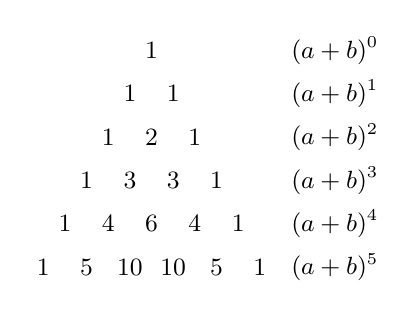
\begin{tikzpicture}[scale=0.55,every node/.style={font=\small}]
\node at (0,0) {1};
\node at (-0.5,-1) {1}; \node at (0.5,-1) {1};
\node at (-1,-2) {1}; \node at (0,-2) {2}; \node at (1,-2) {1};
\node at (-1.5,-3) {1}; \node at (-0.5,-3) {3}; \node at (0.5,-3) {3}; \node at (1.5,-3) {1};
\node at (-2,-4) {1}; \node at (-1,-4) {4}; \node at (0,-4) {6}; \node at (1,-4) {4}; \node at (2,-4) {1};
\node at (-2.5,-5) {1}; \node at (-1.5,-5) {5}; \node at (-0.5,-5) {10}; \node at (0.5,-5) {10}; \node at (1.5,-5) {5}; \node at (2.5,-5) {1};
\node[right] at (3,0) {$(a+b)^0$};
\node[right] at (3,-1) {$(a+b)^1$};
\node[right] at (3,-2) {$(a+b)^2$};
\node[right] at (3,-3) {$(a+b)^3$};
\node[right] at (3,-4) {$(a+b)^4$};
\node[right] at (3,-5) {$(a+b)^5$};
\end{tikzpicture}
\end{center}

\begin{ejbox}{Ejemplo 2.7. Binomio de Newton -- $(a+b)^4$}
$(a+b)^4=a^4+4a^3b+6a^2b^2+4ab^3+b^4$.
\end{ejbox}

\begin{ejbox}{Ejemplo 2.8. Término general}
Encuentra el 4.\textsuperscript{o} término de $(2x-3)^6$. \textit{Solución:} $k=3$: $\binom{6}{3}(2x)^3(-3)^3=20\cdot8x^3\cdot(-27)=-4320x^3$.
\end{ejbox}

\begin{ejbox}{Ejemplo 2.9. Expansión parcial}
Expande $(x+2)^5$ usando el triángulo de Pascal. \textit{Solución:} coeficientes $1,5,10,10,5,1$: $x^5+10x^4+40x^3+80x^2+80x+32$.
\end{ejbox}

\begin{histbox}{Nota: La serie binomial para exponentes negativos}
El Teorema del binomio que vimos arriba ($n\in\mathbb{N}$) produce una suma \textbf{finita}. Cuando el exponente $n$ es un \textbf{entero negativo} (o, en general, no entero), Isaac Newton generalizó la fórmula combinando el coeficiente binomial generalizado
\[ \binom{r}{k} = \frac{r(r-1)(r-2)\cdots(r-k+1)}{k!},\qquad r\in\mathbb{R}, \]
de modo que
\[ (1+x)^r = \sum_{k=0}^{\infty}\binom{r}{k}x^k,\qquad |x|<1. \]
A diferencia del caso $n>0$, esta serie es \textbf{infinita} y solo converge cuando $|x|<1$. Esta es la base de la \emph{serie binomial}, fundamental en cálculo y en aproximaciones numéricas.
\end{histbox}

\begin{ejbox}{Ejemplo 2.9b. Caso $n$ entero negativo}
Obtén los primeros cuatro términos de $(1+x)^{-1}$.\\
\textit{Solución:} $\binom{-1}{k}=(-1)^k$, así
\[ (1+x)^{-1}=1-x+x^2-x^3+\cdots \]
(coincide con la serie geométrica $\sum(-x)^k$, válida para $|x|<1$).
\end{ejbox}

\begin{ejbox}{Ejemplo 2.9c. Otro caso con $n<0$}
Obtén los primeros tres términos de $(1-x)^{-2}$.\\
\textit{Solución:} $\binom{-2}{k}=(-1)^k(k+1)$, así
\[ (1-x)^{-2}=1+2x+3x^2+4x^3+\cdots \]
\end{ejbox}

\textbf{Ejercicios adicionales sobre el Binomio de Newton}

\textit{Caso $n$ entero positivo:}
\begin{enumerate}
\item Expande $(x+1)^6$ usando el triángulo de Pascal.
\item Expande $(2a-b)^5$.
\item Encuentra el 5.\textsuperscript{o} término de $(x+2y)^8$.
\item Encuentra el término que contiene $x^4$ en $(x-3)^{10}$.
\item Encuentra el término central de $(2x+y)^6$.
\item Calcula la suma de los coeficientes de $(3x-1)^5$ (sugerencia: evalúa en $x=1$).
\item Encuentra el coeficiente de $x^3y^4$ en $(x+y)^7$.
\item Usa el binomio de Newton para aproximar $(1.02)^5$ tomando los primeros tres términos de $(1+0.02)^5$.
\end{enumerate}

\textit{Caso $n$ entero negativo (serie binomial):}
\begin{enumerate}
\item Obtén los primeros cuatro términos de $(1+x)^{-3}$.
\item Obtén los primeros tres términos de $(1-2x)^{-1}$.
\item Obtén los primeros cuatro términos de $(1+x)^{-1/2}$ (exponente fraccionario, mismo principio).
\item Usa la serie de $(1+x)^{-1}$ para aproximar $\dfrac{1}{1.05}$ con los primeros tres términos ($x=0.05$).
\item Explica por qué $(1+x)^{-2}$ \emph{no} puede expandirse como una suma finita mediante el triángulo de Pascal, a diferencia de $(1+x)^2$.
\end{enumerate}

\textbf{Respuestas (positivo):} 1. $x^6+6x^5+15x^4+20x^3+15x^2+6x+1$\quad 2. $32a^5-80a^4b+80a^3b^2-40a^2b^3+10ab^4-b^5$\quad 3. $\binom{8}{4}x^4(2y)^4=1120x^4y^4$\quad 4. $\binom{10}{6}x^4(-3)^6=210\cdot729\,x^4=153090x^4$\quad 5. $\binom{6}{3}(2x)^3y^3=160x^3y^3$\quad 6. $2^5=32$\quad 7. $\binom{7}{3}=35$\quad 8. $\approx1+5(0.02)+10(0.02)^2=1.104$.

\textbf{Respuestas (negativo):} 9. $1-3x+6x^2-10x^3$\quad 10. $1+2x+4x^2$\quad 11. $1-\tfrac12x+\tfrac38x^2-\tfrac{5}{16}x^3$\quad 12. $1-0.05+0.0025\approx0.9525$\quad 13. Porque el coeficiente generalizado $\binom{-2}{k}$ nunca se anula, así que la serie tiene infinitos términos no nulos, mientras que para $n>0$ entero, $\binom{n}{k}=0$ si $k>n$.

\section{Factorización}

\begin{center}
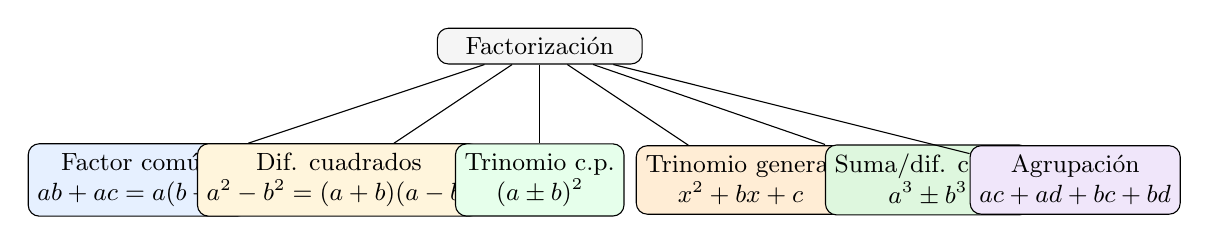
\begin{tikzpicture}[scale=0.85,every node/.style={align=center,font=\small}]
\node[draw,rounded corners,fill=EjColor,minimum width=2.6cm] (root) at (0,0) {Factorización};
\node[draw,rounded corners,fill=DefColor] (a) at (-6,-2) {Factor común\\$ab+ac=a(b+c)$};
\node[draw,rounded corners,fill=ThmColor] (b) at (-3,-2) {Dif. cuadrados\\$a^2-b^2=(a+b)(a-b)$};
\node[draw,rounded corners,fill=PropColor] (c) at (0,-2) {Trinomio c.p.\\$(a\pm b)^2$};
\node[draw,rounded corners,fill=AplColor] (d) at (3,-2) {Trinomio general\\$x^2+bx+c$};
\node[draw,rounded corners,fill=ActColor] (e) at (5.8,-2) {Suma/dif. cubos\\$a^3\pm b^3$};
\node[draw,rounded corners,fill=HistColor] (f) at (8,-2) {Agrupación\\$ac+ad+bc+bd$};
\foreach \n in {a,b,c,d,e,f} \draw (root) -- (\n);
\end{tikzpicture}
\end{center}

\begin{ejbox}{Ejemplo 2.10. Factor común}
$6x^3-9x^2+3x=3x(2x^2-3x+1)=3x(2x-1)(x-1)$.
\end{ejbox}

\begin{ejbox}{Ejemplo 2.11. Diferencia de cuadrados}
$16x^2-25=(4x+5)(4x-5)$.
\end{ejbox}

\begin{ejbox}{Ejemplo 2.12. Trinomio general}
$x^2-7x+12=(x-3)(x-4)$.
\end{ejbox}

\begin{ejbox}{Ejemplo 2.13. Diferencia de cubos}
$8x^3-27=(2x-3)(4x^2+6x+9)$.
\end{ejbox}

\section{Fracciones algebraicas complejas}

\begin{ejbox}{Ejemplo 2.14. Simplificación}
$\dfrac{x^2-4}{x^2-x-2}=\dfrac{(x+2)(x-2)}{(x-2)(x+1)}=\dfrac{x+2}{x+1}$.
\end{ejbox}

\begin{ejbox}{Ejemplo 2.15. Suma de fracciones algebraicas}
$\dfrac{2}{x-1}+\dfrac{3}{x+2}=\dfrac{5x+1}{(x-1)(x+2)}$.
\end{ejbox}

\section{Ecuaciones lineales y cuadráticas}

\begin{center}
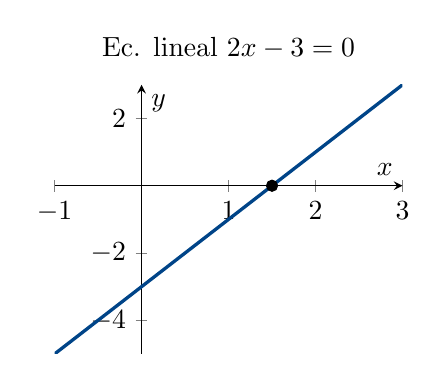
\begin{tikzpicture}
\begin{axis}[width=6cm,height=5cm,xlabel=$x$,ylabel=$y$,title={Ec. lineal $2x-3=0$},axis lines=middle]
\addplot[UANazul,line width=1.2pt,domain=-1:3]{2*x-3};
\addplot[only marks,mark=*] coordinates {(1.5,0)};
\end{axis}
\end{tikzpicture}
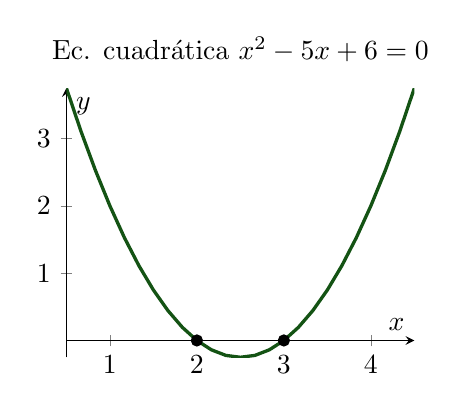
\begin{tikzpicture}
\begin{axis}[width=6cm,height=5cm,xlabel=$x$,ylabel=$y$,title={Ec. cuadrática $x^2-5x+6=0$},axis lines=middle]
\addplot[ForestGreen!60!black,line width=1.2pt,domain=0.5:4.5]{x^2-5*x+6};
\addplot[only marks,mark=*] coordinates {(2,0)(3,0)};
\end{axis}
\end{tikzpicture}
\end{center}

\begin{defbox}{Definición 2.3. Ecuación cuadrática -- fórmula general}
$ax^2+bx+c=0$ ($a\neq0$): $x=\dfrac{-b\pm\sqrt{b^2-4ac}}{2a}$.\\
$\Delta=b^2-4ac$: $\Delta>0$ (dos raíces reales); $\Delta=0$ (raíz doble); $\Delta<0$ (sin raíces reales).
\end{defbox}

\begin{ejbox}{Ejemplo 2.16. Ecuación lineal}
$3(x-2)+5=2x-1\Rightarrow x=0$.
\end{ejbox}

\begin{ejbox}{Ejemplo 2.17. Por factorización}
$x^2-5x+6=0\Rightarrow(x-2)(x-3)=0\Rightarrow x=2$ ó $x=3$.
\end{ejbox}

\begin{ejbox}{Ejemplo 2.18. Fórmula general}
$2x^2-3x-2=0$; $\Delta=25$; $x_1=2$, $x_2=-1/2$.
\end{ejbox}

\section{Racionalización algebraica}

\begin{ejbox}{Ejemplo 2.19. Límite con radical}
Simplifica $\dfrac{x-4}{\sqrt x-2}=\sqrt x+2$.
\end{ejbox}

\section{Ejercicios propuestos}

\begin{enumerate}
\item Suma $(4x^2-3x+2)+(-2x^2+x-5)$.
\item Expande $(3x-2)(2x^2-x+1)$.
\item Aplica: $(4x-3y)^2$.
\item Factoriza: $12x^3-18x^2+6x$.
\item Factoriza: $x^2+2x-15$.
\item Factoriza: $27x^3+8$.
\item Simplifica: $(x^2-1)/(x^2+x)$.
\item Suma: $3/(x-2)+1/(x+3)$.
\item Resuelve: $5(x-1)-3(2x+1)=0$.
\item Resuelve: $3x^2-5x-2=0$.
\item Expande $(a+b)^5$ con el Triángulo de Pascal.
\item Encuentra el término independiente de $(x+1/x)^6$.
\item Factoriza completamente: $x^4-16$.
\item Resuelve: $2/(x-1)=3/(x+2)$.
\item \textit{(Nuevo)} Desarrolla $(2x+5)^2$ y verifica restando $4x^2+25$.
\item \textit{(Nuevo)} Factoriza por agrupación: $x^3+2x^2-9x-18$.
\item \textit{(Nuevo)} Encuentra el 6.\textsuperscript{o} término de $(3x-2y)^9$.
\item \textit{(Nuevo)} Obtén los primeros tres términos de $(1+x)^{-4}$ usando la serie binomial.
\item \textit{(Nuevo)} Resuelve por fórmula general: $4x^2+4x+1=0$ e interpreta el discriminante.
\item \textit{(Nuevo)} Simplifica $\dfrac{x^3-8}{x^2-4}$.
\item \textbf{(Aplicación)} El área de un jardín rectangular es $(x^2+7x+12)$ m$^2$. Factoriza para encontrar posibles dimensiones en términos de $x$.
\item \textbf{(Aplicación)} La ganancia de una empresa (en miles de pesos) se modela con $G(x)=-2x^2+40x-150$, donde $x$ son las unidades vendidas (en cientos). Factoriza para hallar los valores de $x$ donde $G(x)=0$ (puntos de equilibrio).
\item \textbf{(Aplicación)} Un terreno cuadrado de lado $x$ se amplía agregando una franja de 4 m de ancho en dos de sus lados. Expresa el área total como producto notable y desarróllala.
\item \textbf{(Aplicación)} Aproxima $\sqrt[3]{1.03}$ usando los primeros dos términos de la serie binomial de $(1+x)^{1/3}$ con $x=0.03$.
\end{enumerate}

\textbf{Respuestas (1--14):} 1. $2x^2-2x-3$\quad 2. $6x^3-7x^2+5x-2$\quad 3. $16x^2-24xy+9y^2$\quad 4. $6x(2x-1)(x-1)$\quad 5. $(x+5)(x-3)$\quad 6. $(3x+2)(9x^2-6x+4)$\quad 7. $(x-1)/x$\quad 8. $(4x+7)/[(x-2)(x+3)]$\quad 9. $x=-2$\quad 10. $x=2,-1/3$\quad 11. $a^5+5a^4b+10a^3b^2+10a^2b^3+5ab^4+b^5$\quad 12. $\binom{6}{3}=20$\quad 13. $(x^2+4)(x+2)(x-2)$\quad 14. $x=7$.

\textbf{Respuestas (15--23):} 15. $4x^2+20x+25$\quad 16. $(x+2)(x-3)(x+3)$\quad 17. $\binom{9}{5}(3x)^4(-2y)^5=-126\cdot81\cdot32\,x^4y^5=-326592x^4y^5$\quad 18. $1-4x+10x^2$\quad 19. $x=-1/2$ (raíz doble, $\Delta=0$)\quad 20. $\dfrac{x^2+2x+4}{x+2}$\quad 21. $(x+3)(x+4)$, dimensiones $(x+3)$ por $(x+4)$\quad 22. $x=5,15$ (cientos de unidades)\quad 23. $(x+4)(x+4)=x^2+8x+16$ ó depende de la configuración, área total $=x^2+8x+16$ si se amplía en dos lados adyacentes\quad 24. $\approx1+\tfrac{1}{3}(0.03)=1.01$.

% ============================================================
\chapter{Desigualdades}

\section*{Antecedentes: El orden en los números reales}
\addcontentsline{toc}{section}{Antecedentes: El orden en los números reales}

Las desigualdades comparan magnitudes. Conocer el orden de $\mathbb{R}$ es indispensable para determinar dominios de funciones, intervalos de monotonía y regiones de solución.

\begin{center}
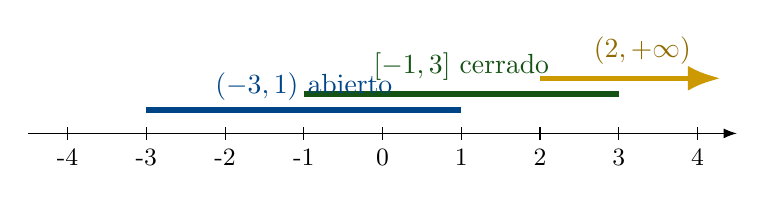
\begin{tikzpicture}
\draw[-{Latex}] (-4.5,0) -- (4.5,0);
\foreach \x in {-4,-3,-2,-1,0,1,2,3,4} \draw (\x,0.08)--(\x,-0.08) node[below]{\small\x};
\draw[UANazul,line width=2pt] (-3,0.3) -- (1,0.3);
\draw[ForestGreen!60!black,line width=2pt] (-1,0.5) -- (3,0.5);
\draw[UANoro,line width=2pt,-{Latex}] (2,0.7) -- (4.3,0.7);
\node[above,UANazul] at (-1,0.3) {$(-3,1)$ abierto};
\node[above,ForestGreen!60!black] at (1,0.55) {$[-1,3]$ cerrado};
\node[above,UANoro!70!black] at (3.3,0.75) {$(2,+\infty)$};
\end{tikzpicture}
\end{center}

\textbf{Objetivo.} Resolver desigualdades lineales, cuadráticas y con valor absoluto, expresando soluciones en notación de intervalo.

\section{Orden de los números reales}

\begin{propbox}{Propiedad 3.1. Propiedades de la desigualdad}
Si $a<b$ y $c>0$: $ac<bc$. Si $c<0$: $ac>bc$ (invierte el signo).
\end{propbox}

\begin{defbox}{Definición 3.1. Tipos de intervalo}
\begin{center}
\begin{tabular}{lll}
\textbf{Notación} & \textbf{Inecuación} & \textbf{Tipo}\\\hline
$(a,b)$ & $a<x<b$ & abierto\\
$[a,b]$ & $a\leq x\leq b$ & cerrado\\
$[a,b)$ & $a\leq x<b$ & semiabierto\\
$(a,\infty)$ & $x>a$ & semirrecta\\
$(-\infty,b]$ & $x\leq b$ & semirrecta
\end{tabular}
\end{center}
\end{defbox}

\section{Desigualdades lineales}

\begin{ejbox}{Ejemplo 3.1. Simple}
$3x-7>2\Rightarrow x>3$. Solución: $(3,+\infty)$.
\end{ejbox}

\begin{ejbox}{Ejemplo 3.2. Doble}
$-1\leq2x+3<7\Rightarrow-2\leq x<2$. Solución: $[-2,2)$.
\end{ejbox}

\begin{ejbox}{Ejemplo 3.3. Con fracciones}
$(x-1)/2\geq(x+3)/4\Rightarrow x\geq5$. Solución: $[5,+\infty)$.
\end{ejbox}

\section{Desigualdades con valor absoluto}

\begin{propbox}{Propiedad 3.2. Reglas fundamentales}
$|x|<k\Leftrightarrow-k<x<k$;\qquad $|x|>k\Leftrightarrow x<-k$ ó $x>k$.
\end{propbox}

\begin{ejbox}{Ejemplo 3.4. Tipo $|A|<k$}
$|2x-1|<5\Rightarrow-2<x<3$. Solución: $(-2,3)$.
\end{ejbox}

\begin{ejbox}{Ejemplo 3.5. Tipo $|A|>k$}
$|x+3|>2\Rightarrow x<-5$ ó $x>-1$. Solución: $(-\infty,-5)\cup(-1,+\infty)$.
\end{ejbox}

\begin{ejbox}{Ejemplo 3.6. Compuesta}
$1\leq|3x-6|\leq9\Rightarrow[-1,5/3]\cup[7/3,5]$.
\end{ejbox}

\section{Desigualdades cuadráticas}

\begin{center}
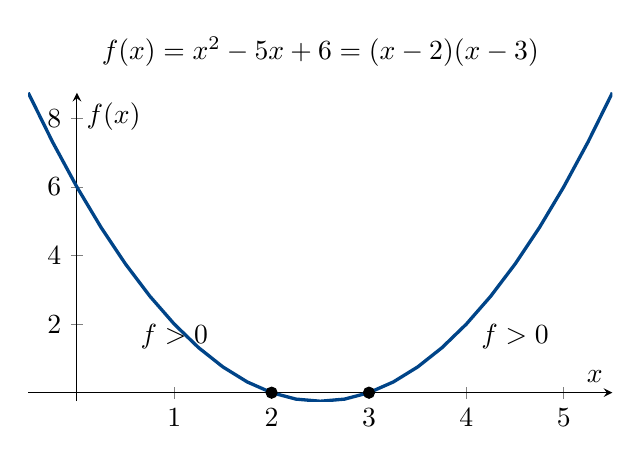
\begin{tikzpicture}
\begin{axis}[width=9cm,height=5.5cm,xlabel=$x$,ylabel=$f(x)$,axis lines=middle,
title={$f(x)=x^2-5x+6=(x-2)(x-3)$}]
\addplot[UANazul,line width=1.2pt,domain=-0.5:5.5]{x^2-5*x+6};
\addplot[only marks,mark=*] coordinates {(2,0)(3,0)};
\node[above] at (axis cs:1,1) {$f>0$};
\node[below] at (axis cs:2.5,-0.5) {$f<0$};
\node[above] at (axis cs:4.5,1) {$f>0$};
\end{axis}
\end{tikzpicture}
\end{center}

\begin{ejbox}{Ejemplo 3.7. $f<0$}
$x^2-5x+6<0\Rightarrow(x-2)(x-3)<0\Rightarrow(2,3)$.
\end{ejbox}

\begin{ejbox}{Ejemplo 3.8. $f\geq0$}
$x^2-2x-3\geq0\Rightarrow(x-3)(x+1)\geq0\Rightarrow(-\infty,-1]\cup[3,+\infty)$.
\end{ejbox}

\begin{ejbox}{Ejemplo 3.9. Sin raíces reales}
$x^2+2x+5>0$: $\Delta<0$, parábola arriba del eje. Solución: $\mathbb{R}$.
\end{ejbox}

\begin{aplbox}{Problema de aplicación 3.1. Temperatura}
La escala Celsius y Fahrenheit se relacionan por $F=\tfrac95C+32$. ¿Para qué valores de $C$ se cumple que $F$ está entre $68^\circ$ y $104^\circ$?\\
\textit{Solución:} $68\leq\tfrac95C+32\leq104\Rightarrow20\leq C\leq40$.
\end{aplbox}

\begin{aplbox}{Problema de aplicación 3.2. Costos e ingresos}
Una empresa produce $x$ artículos con costo $C(x)=500+8x$ e ingreso $I(x)=20x$. ¿Para qué cantidad de artículos la empresa obtiene utilidad (ingreso mayor al costo)?\\
\textit{Solución:} $20x>500+8x\Rightarrow12x>500\Rightarrow x>41.67$, es decir, a partir de $42$ artículos.
\end{aplbox}

\section{Ejercicios propuestos}

\begin{enumerate}
\item Resuelve y grafica: $4x+3\leq15$.
\item Resuelve: $-3<2x-1<9$.
\item Resuelve: $(3x-1)/2>(x+3)/4$.
\item Resuelve: $|x-2|\leq4$.
\item Resuelve: $|2x+3|>7$.
\item Resuelve: $|x-1|\leq0$.
\item Resuelve: $x^2-x-12\leq0$.
\item Resuelve: $2x^2+x-1>0$.
\item Resuelve: $x^2+6x+9\geq0$.
\item Resuelve: $x^2+1<0$.
\item \textit{(Nuevo)} Resuelve: $\dfrac{x-3}{x+2}\geq0$ (desigualdad racional, considera el dominio).
\item \textit{(Nuevo)} Resuelve: $|5-2x|\geq3$.
\item \textit{(Nuevo)} Resuelve: $x^2-4x>0$ e interpreta gráficamente.
\item \textit{(Nuevo)} Resuelve el sistema: $x+1>0$ y $x-4\leq0$ simultáneamente.
\item \textbf{(Aplicación)} Un fabricante requiere que el diámetro de una pieza esté dentro de $0.02$ mm del valor nominal de $15$ mm. Expresa esto como una desigualdad con valor absoluto y resuélvela.
\item \textbf{(Aplicación)} La altura de un proyectil es $h(t)=-5t^2+20t$ (metros, $t$ en segundos). ¿Durante qué intervalo de tiempo el proyectil está a más de $15$ m de altura?
\end{enumerate}

\textbf{Respuestas (1--10):} 1. $(-\infty,3]$\quad 2. $(-1,5)$\quad 3. $(7/4,+\infty)$\quad 4. $[-2,6]$\quad 5. $(-\infty,-5)\cup(2,+\infty)$\quad 6. $\{1\}$\quad 7. $[-3,4]$\quad 8. $(-\infty,-1)\cup(1/2,+\infty)$\quad 9. $\mathbb{R}$\quad 10. Sin solución real.

\textbf{Respuestas (11--16):} 11. $(-\infty,-2)\cup[3,+\infty)$\quad 12. $x\leq1$ ó $x\geq4$\quad 13. $(-\infty,0)\cup(4,+\infty)$\quad 14. $(-1,4]$\quad 15. $|d-15|\leq0.02\Rightarrow d\in[14.98,15.02]$ mm\quad 16. $1<t<3$ segundos.

% ============================================================
\chapter{Funciones}

\section*{Antecedentes: Del conjunto al par ordenado}
\addcontentsline{toc}{section}{Antecedentes: Del conjunto al par ordenado}

Una función formaliza la idea de ``dependencia'': el área de un círculo depende de su radio; la temperatura de un cuerpo depende del tiempo. La siguiente ilustración contrasta una relación que es función con una que no lo es.

\begin{center}
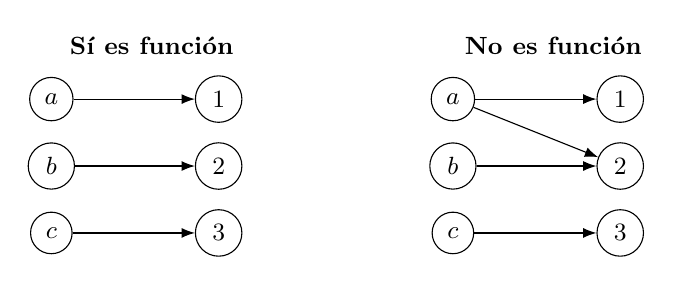
\begin{tikzpicture}[scale=0.85,every node/.style={font=\small}]
\node at (-2,2.3) {\textbf{Sí es función}};
\node[draw,circle] (a1) at (-3.5,1.5) {$a$};
\node[draw,circle] (b1) at (-3.5,0.5) {$b$};
\node[draw,circle] (c1) at (-3.5,-0.5) {$c$};
\node[draw,circle] (1a) at (-1,1.5) {$1$};
\node[draw,circle] (2a) at (-1,0.5) {$2$};
\node[draw,circle] (3a) at (-1,-0.5) {$3$};
\draw[-{Latex}] (a1)--(1a); \draw[-{Latex}] (b1)--(2a); \draw[-{Latex}] (c1)--(3a);
\node at (4,2.3) {\textbf{No es función}};
\node[draw,circle] (a2) at (2.5,1.5) {$a$};
\node[draw,circle] (b2) at (2.5,0.5) {$b$};
\node[draw,circle] (c2) at (2.5,-0.5) {$c$};
\node[draw,circle] (1b) at (5,1.5) {$1$};
\node[draw,circle] (2b) at (5,0.5) {$2$};
\node[draw,circle] (3b) at (5,-0.5) {$3$};
\draw[-{Latex}] (a2)--(1b); \draw[-{Latex}] (a2)--(2b); \draw[-{Latex}] (b2)--(2b); \draw[-{Latex}] (c2)--(3b);
\end{tikzpicture}
\end{center}

\textbf{Objetivo.} Definir y clasificar funciones, determinar dominio y rango y analizar las familias de funciones elementales.

\begin{histbox}{Importancia y aplicaciones del concepto de función}
El concepto de función es uno de los pilares de las matemáticas modernas: permite describir con precisión cómo una cantidad depende de otra. Su importancia es transversal a las ciencias y la ingeniería:
\begin{itemize}
\item En \textbf{física}, la posición de un objeto en caída libre se modela como función del tiempo, $h(t)=h_0-\tfrac12gt^2$.
\item En \textbf{economía}, la demanda de un producto es función de su precio, y las funciones de costo e ingreso permiten determinar puntos de equilibrio y maximizar utilidades.
\item En \textbf{biología}, el crecimiento poblacional se modela con funciones exponenciales o logísticas.
\item En \textbf{ingeniería}, las señales eléctricas, la transferencia de calor y el comportamiento estructural se describen mediante funciones de una o varias variables.
\item En \textbf{ciencias de la computación}, toda función matemática es la base conceptual de las funciones y subrutinas de programación.
\end{itemize}
Sin el concepto de función, sería imposible construir modelos predictivos: dado un valor de entrada, la función garantiza un único valor de salida, lo que permite hacer ciencia reproducible.
\end{histbox}

\section{Conceptos generales}

\begin{defbox}{Definición 4.1. Función}
$f:A\to B$ asigna a cada $x\in A$ exactamente un $f(x)\in B$. $A=\mathrm{Dom}\,f$; $\mathrm{Ran}\,f=\{f(x):x\in A\}$.
\end{defbox}

\begin{ejbox}{Ejemplo 4.1. Dominio}
$f(x)=\dfrac{\sqrt{x+3}}{x-2}$: $\mathrm{Dom}\,f=[-3,2)\cup(2,+\infty)$.
\end{ejbox}

\begin{ejbox}{Ejemplo 4.2. Evaluación}
$f(x)=3x^2-2x+1$: $f(0)=1$; $f(-1)=6$; $f(a+1)=3a^2+4a+2$.
\end{ejbox}

\begin{actbox}{Actividad: Diferenciar función de relación}
Una \textbf{relación} es cualquier conjunto de pares ordenados; una \textbf{función} es una relación en la que cada elemento del dominio tiene exactamente \emph{una} imagen (criterio de la recta vertical en su gráfica).\\[4pt]
\textbf{Instrucciones.} Para cada inciso, determina si la relación dada es función. Justifica usando la definición o el criterio de la recta vertical.
\begin{enumerate}[label=(\alph*)]
\item $R_1=\{(1,2),(2,4),(3,6),(4,8)\}$.
\item $R_2=\{(1,2),(1,-2),(4,3)\}$.
\item La circunferencia $x^2+y^2=9$.
\item $y=2x-5$.
\item El conjunto de pares (alumno, calificación) en un grupo, donde cada alumno solo presenta un examen.
\item El conjunto de pares (persona, número telefónico) en una empresa donde algunos empleados tienen dos teléfonos.
\item $y^2=x$.
\item $f(x)=|x|$.
\end{enumerate}
\textit{Respuestas:} (a) Función ($1\to2$ único, etc.) (b) No es función: $1$ tiene dos imágenes ($2$ y $-2$). (c) No es función: falla la prueba de la recta vertical (para cada $x\in(-3,3)$ hay dos valores de $y$). (d) Función: a cada $x$ le corresponde un único $y$. (e) Función. (f) No es función si algún empleado tiene dos teléfonos asociados. (g) No es función: para $x>0$ hay dos valores de $y$ ($\pm\sqrt x$). (h) Función.
\end{actbox}

\section{Formas de representar una función}

\begin{center}
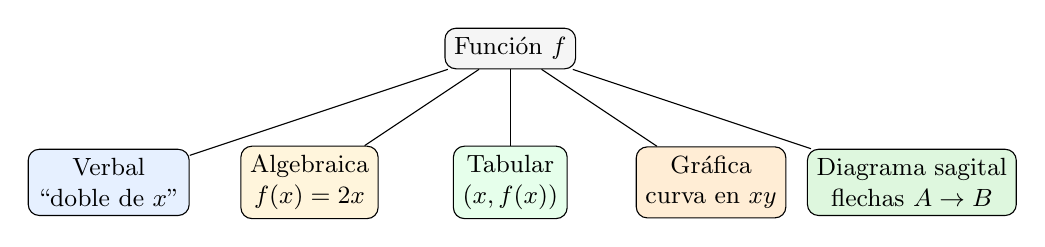
\begin{tikzpicture}[scale=0.85,every node/.style={align=center,font=\small}]
\node[draw,rounded corners,fill=EjColor] (root) at (0,0) {Función $f$};
\node[draw,rounded corners,fill=DefColor] (a) at (-6,-2) {Verbal\\``doble de $x$''};
\node[draw,rounded corners,fill=ThmColor] (b) at (-3,-2) {Algebraica\\$f(x)=2x$};
\node[draw,rounded corners,fill=PropColor] (c) at (0,-2) {Tabular\\$(x,f(x))$};
\node[draw,rounded corners,fill=AplColor] (d) at (3,-2) {Gráfica\\curva en $xy$};
\node[draw,rounded corners,fill=ActColor] (e) at (6,-2) {Diagrama sagital\\flechas $A\to B$};
\foreach \n in {a,b,c,d,e} \draw (root) -- (\n);
\end{tikzpicture}
\end{center}

\section{Clasificación de funciones}
\subsection{Funciones lineales}

\begin{defbox}{Definición 4.2. Función lineal}
$f(x)=mx+b$. Gráfica: recta con pendiente $m$ e intercepto $b$.
\end{defbox}

\begin{center}
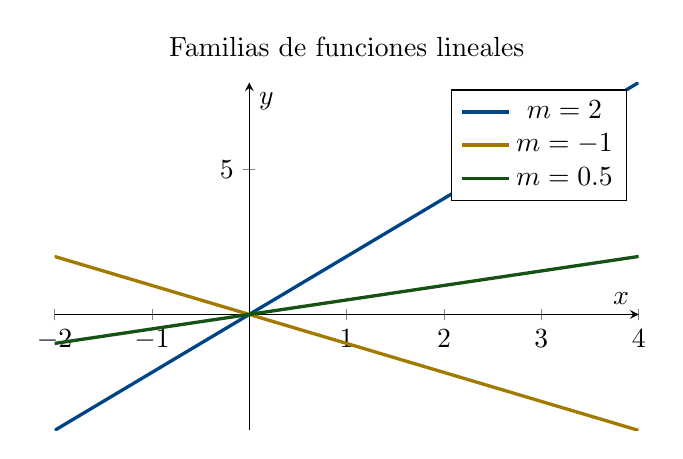
\begin{tikzpicture}
\begin{axis}[width=9cm,height=6cm,xlabel=$x$,ylabel=$y$,axis lines=middle,title={Familias de funciones lineales}]
\addplot[UANazul,line width=1.2pt,domain=-2:4]{2*x};
\addplot[UANoro!80!black,line width=1.2pt,domain=-2:4]{-x};
\addplot[ForestGreen!60!black,line width=1.2pt,domain=-2:4]{0.5*x};
\legend{$m=2$,$m=-1$,$m=0.5$}
\end{axis}
\end{tikzpicture}
\end{center}

\subsection{Funciones cuadráticas}

\begin{defbox}{Definición 4.3. Función cuadrática}
$f(x)=ax^2+bx+c$. Vértice: $V=(-b/(2a),f(-b/(2a)))$. Eje de simetría: $x=-b/(2a)$.
\end{defbox}

\begin{center}
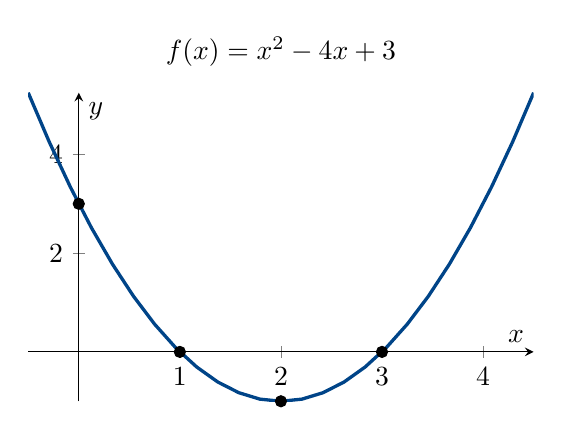
\begin{tikzpicture}
\begin{axis}[width=8cm,height=5.5cm,xlabel=$x$,ylabel=$y$,axis lines=middle,title={$f(x)=x^2-4x+3$}]
\addplot[UANazul,line width=1.2pt,domain=-0.5:4.5]{x^2-4*x+3};
\addplot[only marks,mark=*] coordinates {(1,0)(3,0)(0,3)(2,-1)};
\node[below] at (axis cs:2,-1) {$V(2,-1)$};
\end{axis}
\end{tikzpicture}
\end{center}

\subsection{Funciones potenciales y polinomiales}

\begin{center}
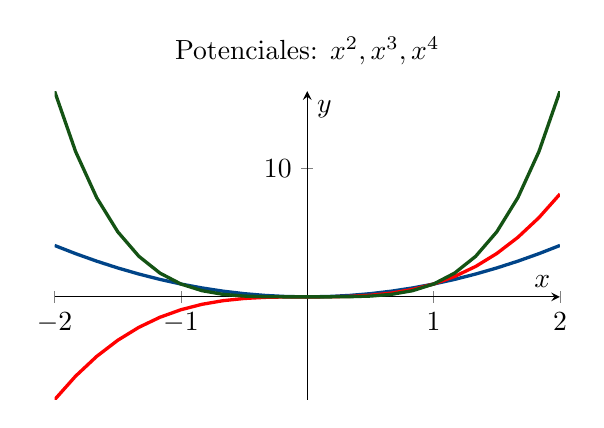
\begin{tikzpicture}
\begin{axis}[width=8cm,height=5.5cm,xlabel=$x$,ylabel=$y$,axis lines=middle,title={Potenciales: $x^2,x^3,x^4$}]
\addplot[UANazul,line width=1.2pt,domain=-2:2]{x^2};
\addplot[red,line width=1.2pt,domain=-2:2]{x^3};
\addplot[ForestGreen!60!black,line width=1.2pt,domain=-2:2]{x^4};
\end{axis}
\end{tikzpicture}
\end{center}

\subsection{Funciones racionales}

\begin{center}
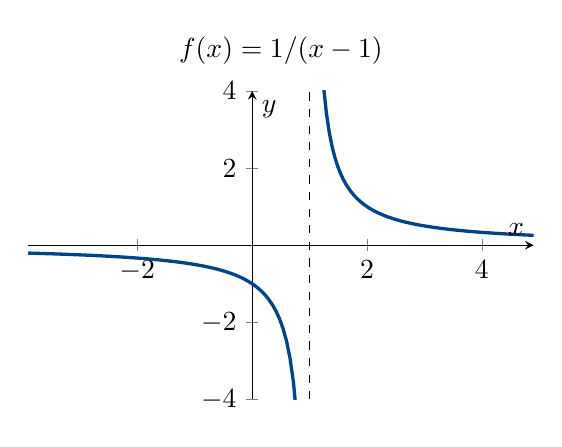
\begin{tikzpicture}
\begin{axis}[width=8cm,height=5.5cm,xlabel=$x$,ylabel=$y$,axis lines=middle,title={$f(x)=1/(x-1)$},ymin=-4,ymax=4]
\addplot[UANazul,line width=1.2pt,domain=-3.9:0.9,samples=80]{1/(x-1)};
\addplot[UANazul,line width=1.2pt,domain=1.1:4.9,samples=80]{1/(x-1)};
\draw[dashed] (axis cs:1,-4) -- (axis cs:1,4);
\end{axis}
\end{tikzpicture}
\end{center}

\subsection{Funciones trigonométricas}

\begin{center}
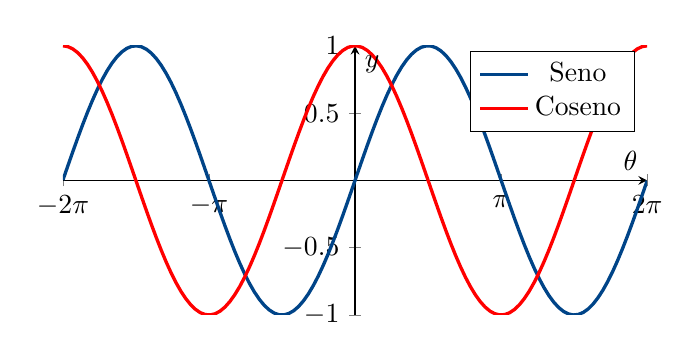
\begin{tikzpicture}
\begin{axis}[width=9cm,height=5cm,xlabel=$\theta$,ylabel=$y$,axis lines=middle,
xtick={-6.28,-3.14,0,3.14,6.28},xticklabels={$-2\pi$,$-\pi$,$0$,$\pi$,$2\pi$}]
\addplot[UANazul,line width=1.2pt,domain=-6.28:6.28,samples=120]{sin(deg(x))};
\addplot[red,line width=1.2pt,domain=-6.28:6.28,samples=120]{cos(deg(x))};
\legend{Seno,Coseno}
\end{axis}
\end{tikzpicture}
\end{center}

\begin{propbox}{Propiedad 4.1. Identidades pitagóricas}
$\sen^2\theta+\cos^2\theta=1$;\quad $1+\tg^2\theta=\sec^2\theta$;\quad $1+\cotg^2\theta=\csc^2\theta$.
\end{propbox}

\begin{ejbox}{Ejemplo 4.3. Evaluación trigonométrica}
$\sen30^\circ=1/2$; $\cos(\pi/3)=1/2$; $\tg45^\circ=1$.
\end{ejbox}

\begin{ejbox}{Ejemplo 4.4. Uso de identidades}
$\sen\theta=3/5$, primer cuadrante: $\cos\theta=4/5$; $\tg\theta=3/4$.
\end{ejbox}

\begin{aplbox}{Problemas de aplicación}
\textbf{a)} El costo de producir $x$ unidades es $C(x)=1500+12x$ y el ingreso es $I(x)=25x$. Encuentra el punto de equilibrio.\\
\textit{Solución:} $1500+12x=25x\Rightarrow x=\tfrac{1500}{13}\approx115$ unidades.\\[4pt]
\textbf{b)} La altura de un proyectil lanzado verticalmente es $h(t)=-4.9t^2+30t$. ¿En qué instante alcanza su altura máxima y cuál es?\\
\textit{Solución:} vértice en $t=-30/(2(-4.9))\approx3.06$ s, $h\approx45.9$ m.\\[4pt]
\textbf{c)} La población de bacterias se modela con $P(t)=200(1.15)^t$. ¿Cuál es la población a las 5 horas?\\
\textit{Solución:} $P(5)=200(1.15)^5\approx402$ bacterias.
\end{aplbox}

\section{Ejercicios propuestos}

\begin{enumerate}
\item Dominio de $f(x)=\sqrt{4-x^2}$.
\item Dominio de $g(x)=(x+1)/(x^2-4)$.
\item Si $h(x)=x^2-3x$, calcula $h(0),h(2),h(a-1)$.
\item Grafica $f(x)=-2x+4$ e identifica interceptos.
\item Para $f(x)=-x^2+4x-3$, halla vértice e interceptos.
\item Determina si $f(x)=x^4$ es par, impar o ninguna.
\item Dominio de $f(x)=\sqrt x/(x^2-x-6)$.
\item Evalúa $P(x)=x^3-2x^2+x-5$ en $x=-1$ (Horner).
\item Asíntotas de $f(x)=(2x-1)/(x+3)$.
\item Simplifica $(\sen^2\theta-1)/\cos\theta$.
\item Si $\cos\theta=-5/13$, $\theta$ en 2.\textsuperscript{o} cuadrante, halla todas las trig.
\item Grafica $\tg(x)$ en $(-\pi/2,\pi/2)$.
\item \textit{(Nuevo)} Determina si $g=\{(x,y):x=y^2\}$ es función. Justifica.
\item \textit{(Nuevo)} Sea $f(x)=2x-3$ y $g(x)=x^2+1$. Calcula $(f\circ g)(x)$ y $(g\circ f)(x)$.
\item \textit{(Nuevo)} Determina si $f(x)=x^3-x$ es par, impar o ninguna, mediante $f(-x)$.
\item \textit{(Nuevo)} Encuentra el dominio y rango de $f(x)=\sqrt{9-x^2}$.
\item \textbf{(Aplicación)} El área de un rectángulo de perímetro fijo $40$ m se expresa como $A(x)=x(20-x)$, donde $x$ es la base. ¿Para qué valor de $x$ el área es máxima?
\item \textbf{(Aplicación)} Una compañía de telefonía cobra \$150 de renta más \$2 por minuto. Expresa el costo total $C$ como función de los minutos $m$ y calcula $C(120)$.
\item \textbf{(Aplicación)} La distancia de frenado de un automóvil (en metros) se aproxima con $d(v)=0.0056v^2+0.14v$, donde $v$ es la velocidad en km/h. Calcula $d(80)$.
\end{enumerate}

\textbf{Respuestas (1--12):} 1. $[-2,2]$\quad 2. $\mathbb{R}\setminus\{-2,2\}$\quad 3. $0;-2;a^2-5a+4$\quad 4. $x$-int: $2$; $y$-int: $4$\quad 5. $V(2,1)$; raíces $1,3$\quad 6. Par\quad 7. $[0,2)\cup(2,3)\cup(3,+\infty)$\quad 8. $-9$\quad 9. AV: $x=-3$; AH: $y=2$\quad 10. $-\sen\theta$\quad 11. $\sen\theta=12/13,\tg\theta=-12/5$\quad 12. AV: $x=\pm\pi/2$.

\textbf{Respuestas (13--19):} 13. No es función: para $x>0$ hay dos valores de $y$\quad 14. $(f\circ g)(x)=2x^2-1$; $(g\circ f)(x)=4x^2-12x+10$\quad 15. Impar: $f(-x)=-f(x)$\quad 16. Dom $=[-3,3]$, Ran $=[0,3]$\quad 17. $x=10$ m (área máxima $=100$ m$^2$)\quad 18. $C(m)=150+2m$; $C(120)=\$390$\quad 19. $d(80)=0.0056(6400)+0.14(80)=35.84+11.2=47.04$ m.

% ============================================================
\chapter{Logaritmos}

\section*{Antecedentes: La función inversa de la exponencial}
\addcontentsline{toc}{section}{Antecedentes: La función inversa de la exponencial}

Si la exponencial ``sube'' ($b^x$), el logaritmo ``invierte'' ese proceso. Su utilidad práctica abarca: escalas de decibeles, pH, escala Richter, interés compuesto y modelos de crecimiento/decaimiento.

\begin{center}
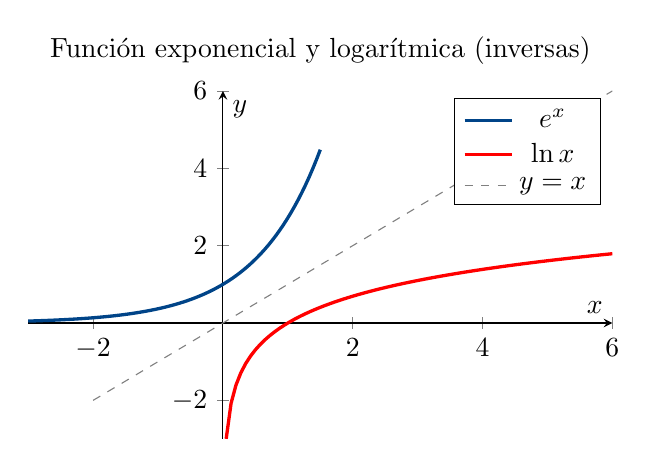
\begin{tikzpicture}
\begin{axis}[width=9cm,height=6cm,xlabel=$x$,ylabel=$y$,axis lines=middle,
title={Función exponencial y logarítmica (inversas)}]
\addplot[UANazul,line width=1.2pt,domain=-3:1.5,samples=80]{exp(x)};
\addplot[red,line width=1.2pt,domain=0.05:6,samples=80]{ln(x)};
\addplot[gray,dashed,domain=-2:6]{x};
\legend{$e^x$,$\ln x$,$y=x$}
\end{axis}
\end{tikzpicture}
\end{center}

\begin{center}
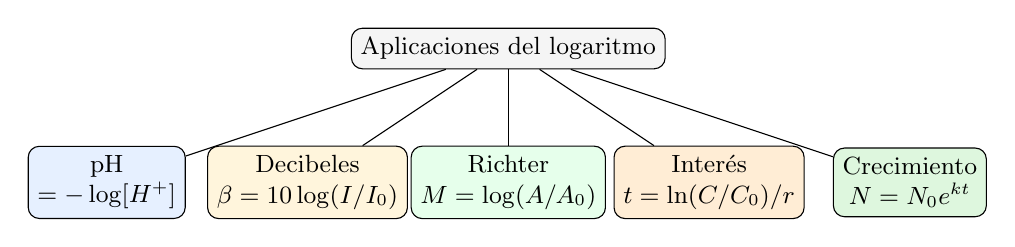
\begin{tikzpicture}[scale=0.85,every node/.style={align=center,font=\small}]
\node[draw,rounded corners,fill=EjColor] (root) at (0,0) {Aplicaciones del logaritmo};
\node[draw,rounded corners,fill=DefColor] (a) at (-6,-2) {pH\\$=-\log[H^+]$};
\node[draw,rounded corners,fill=ThmColor] (b) at (-3,-2) {Decibeles\\$\beta=10\log(I/I_0)$};
\node[draw,rounded corners,fill=PropColor] (c) at (0,-2) {Richter\\$M=\log(A/A_0)$};
\node[draw,rounded corners,fill=AplColor] (d) at (3,-2) {Interés\\$t=\ln(C/C_0)/r$};
\node[draw,rounded corners,fill=ActColor] (e) at (6,-2) {Crecimiento\\$N=N_0e^{kt}$};
\foreach \n in {a,b,c,d,e} \draw (root) -- (\n);
\end{tikzpicture}
\end{center}

\textbf{Objetivo.} Definir el logaritmo, aplicar sus propiedades y resolver ecuaciones logarítmicas y exponenciales.

\begin{histbox}{Antecedentes históricos y la importancia de los logaritmos}
\textbf{Origen.} Los logaritmos nacieron a principios del siglo XVII como una herramienta de cálculo, en una época sin calculadoras, para simplificar multiplicaciones, divisiones, potencias y raíces de números muy grandes (frecuentes en astronomía y navegación), convirtiéndolos en sumas y restas. El matemático escocés \textbf{John Napier (Neper)} publicó en 1614 su obra \emph{Mirifici Logarithmorum Canonis Descriptio}, donde introdujo el concepto y construyó las primeras tablas de logaritmos, fruto de casi veinte años de trabajo.\\[4pt]
Poco después, el matemático inglés \textbf{Henry Briggs} visitó a Napier y juntos propusieron una versión más práctica: el \textbf{logaritmo de base 10} (logaritmo común o ``briggsiano''), publicado en tablas que se usaron durante más de tres siglos en ingeniería, astronomía y navegación, hasta la llegada de las calculadoras electrónicas.\\[4pt]
\textbf{La importancia de Euler.} Fue \textbf{Leonhard Euler}, en el siglo XVIII, quien estableció con rigor la relación entre los logaritmos y las funciones exponenciales, mostrando que el logaritmo es la función \emph{inversa} de la exponencial. Euler también introdujo y popularizó la constante $e\approx2.71828\ldots$ (conocida como el número de Euler), base del logaritmo natural $\ln x = \log_e x$. Gracias a Euler, los logaritmos dejaron de ser solo una herramienta de cálculo manual y se convirtieron en un objeto central del análisis matemático, fundamental para el cálculo diferencial e integral, las ecuaciones diferenciales y la modelación de fenómenos de crecimiento y decaimiento.\\[4pt]
\textbf{Aplicaciones actuales.} Hoy los logaritmos son indispensables en: la escala de pH en química, la escala de decibeles en acústica, la escala de Richter en sismología, el cálculo de interés compuesto e inversiones financieras, los modelos de crecimiento poblacional y decaimiento radiactivo, la teoría de la información (bits, entropía), y los algoritmos computacionales (complejidad logarítmica, búsqueda binaria).
\end{histbox}

\section{Definición}

\begin{defbox}{Definición 5.1. Logaritmo}
$\log_b x=y\Leftrightarrow b^y=x$ ($b>0$, $b\neq1$, $x>0$).\\
$\log_{10}x=\log x$;\quad $\log_e x=\ln x$ ($e\approx2.71828$).
\end{defbox}

\begin{ejbox}{Ejemplo 5.1. Conversión}
$\log_2 8=3\Leftrightarrow2^3=8$.
\end{ejbox}

\begin{ejbox}{Ejemplo 5.2. Evaluación}
$\log_5 25=2$; $\log_{1/2}8=-3$; $\ln e^3=3$.
\end{ejbox}

\section{Propiedades}

\begin{propbox}{Propiedad 5.1. Propiedades de los logaritmos}
\begin{center}
\begin{tabular}{lll}
\textbf{Propiedad} & \textbf{Fórmula} & \textbf{Ejemplo}\\\hline
Producto & $\log_b(MN)=\log_bM+\log_bN$ & $\log6=\log2+\log3$\\
Cociente & $\log_b(M/N)=\log_bM-\log_bN$ & $\ln(e^2/3)=2-\ln3$\\
Potencia & $\log_bM^p=p\log_bM$ & $\log(100^3)=6$\\
Neutros & $\log_bb=1;\log_b1=0$ & $\ln e=1;\log1=0$\\
Inversos & $b^{\log_bM}=M;\log_bb^x=x$ & $10^{\log7}=7$\\
Cambio de base & $\log_bM=\dfrac{\ln M}{\ln b}$ & $\log_750\approx2.01$
\end{tabular}
\end{center}
\end{propbox}

\begin{center}
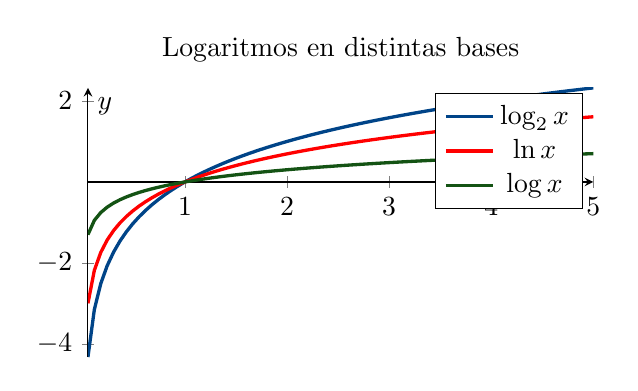
\begin{tikzpicture}
\begin{axis}[width=8cm,height=5cm,xlabel=$x$,ylabel=$y$,axis lines=middle,title={Logaritmos en distintas bases}]
\addplot[UANazul,line width=1.2pt,domain=0.05:5,samples=80]{ln(x)/ln(2)};
\addplot[red,line width=1.2pt,domain=0.05:5,samples=80]{ln(x)};
\addplot[ForestGreen!60!black,line width=1.2pt,domain=0.05:5,samples=80]{ln(x)/ln(10)};
\legend{$\log_2x$,$\ln x$,$\log x$}
\end{axis}
\end{tikzpicture}
\end{center}

\begin{ejbox}{Ejemplo 5.3. Expansión}
$\log\left(\dfrac{x^2\sqrt y}{z^3}\right)=2\log x+\tfrac12\log y-3\log z$.
\end{ejbox}

\begin{ejbox}{Ejemplo 5.4. Contracción}
$3\ln x-\ln(x+1)+2\ln y=\ln\dfrac{x^3y^2}{x+1}$.
\end{ejbox}

\begin{ejbox}{Ejemplo 5.5. Cambio de base}
$\log_750=\dfrac{\ln50}{\ln7}\approx2.011$.
\end{ejbox}

\section{Ecuaciones logarítmicas}

\begin{propbox}{Propiedad 5.2. Estrategia}
(1) Aislar/combinar logaritmos. (2) Convertir: $\log_bA=c\Rightarrow A=b^c$. (3) Verificar dominio ($A>0$).
\end{propbox}

\begin{ejbox}{Ejemplo 5.6. Simple}
$\log_3(2x-1)=4\Rightarrow2x-1=81\Rightarrow x=41$.
\end{ejbox}

\begin{ejbox}{Ejemplo 5.7. Dos logaritmos}
$\log(x+2)+\log(x-1)=1\Rightarrow(x+2)(x-1)=10\Rightarrow x=3$.
\end{ejbox}

\begin{ejbox}{Ejemplo 5.8. Logarítmica avanzada}
$\ln(x^2-1)-\ln(x+1)=\ln2\Rightarrow x-1=2\Rightarrow x=3$.
\end{ejbox}

\textbf{Ejercicios adicionales: ecuaciones con la misma base}
\begin{enumerate}
\item $\log_2(x+5)=\log_2(3x-1)$.
\item $\ln(2x+3)=\ln(x+9)$.
\item $\log_5(x^2-1)=\log_5(2x+2)$.
\item $\log_3(4x)-\log_3(x-1)=\log_3 8$.
\item $2\log_4(x)=\log_4(3x+4)$.
\end{enumerate}
\textit{Idea clave:} si $\log_bA=\log_bB$ entonces $A=B$ (con $A,B>0$), pues el logaritmo es una función inyectiva en una misma base.

\textbf{Ejercicios adicionales: ecuaciones con bases diferentes}
\begin{enumerate}
\item $\log_2 x=\log_5 25$ (evalúa el lado derecho y despeja $x$).
\item $3^{x}=2^{x+1}$ (aplica logaritmo en ambos lados).
\item $\log_3 x=\log_9 16$ (usa cambio de base para igualar bases).
\item $5^{2x-1}=7^{x}$.
\item $\log_2(x)=\log_4(x+6)$ (sugerencia: expresa $\log_4$ en términos de $\log_2$).
\end{enumerate}
\textit{Idea clave:} cuando las bases son distintas, conviene usar la fórmula de cambio de base $\log_bM=\ln M/\ln b$ para reducir todo a una sola base, o aplicar logaritmo natural a ambos lados de una ecuación exponencial.

\textbf{Respuestas (misma base):} 1. $x=3$\quad 2. $x=6$\quad 3. $x=3$ (se descarta $x=-1$ por dominio)\quad 4. $x=2$\quad 5. $x=4$ (se descarta $x=-4/3$).

\textbf{Respuestas (bases diferentes):} 6. $\log_5 25=2\Rightarrow x=4$\quad 7. $x\ln3=(x+1)\ln2\Rightarrow x=\dfrac{\ln2}{\ln3-\ln2}\approx1.71$\quad 8. $\log_9 16=\dfrac{\ln16}{\ln9}\Rightarrow x=3^{\ln16/\ln9}\approx6.35$\quad 9. $(2x-1)\ln5=x\ln7\Rightarrow x=\dfrac{\ln5}{2\ln5-\ln7}\approx2.31$\quad 10. $\log_4(x+6)=\tfrac12\log_2(x+6)$, entonces $\log_2x=\tfrac12\log_2(x+6)\Rightarrow x^2=x+6\Rightarrow x=3$ (se descarta $x=-2$).

\section{Ecuaciones exponenciales}

\begin{ejbox}{Ejemplo 5.9. Misma base}
$4^{x+1}=8^{x-2}\Rightarrow2^{2x+2}=2^{3x-6}\Rightarrow x=8$.
\end{ejbox}

\begin{ejbox}{Ejemplo 5.10. Bases distintas}
$3^x=7\Rightarrow x=\ln7/\ln3\approx1.771$.
\end{ejbox}

\begin{ejbox}{Ejemplo 5.11. Ecuación cuadrática exponencial}
$e^{2x}-5e^x+6=0$; $u=e^x$; $(u-2)(u-3)=0$; $x=\ln2$ ó $x=\ln3$.
\end{ejbox}

\begin{ejbox}{Ejemplo 5.12. Aplicación: Decaimiento radiactivo}
La vida media del C-14 es 5730 años. Un hueso tiene 30\% del C-14 original. ¿Cuántos años tiene?\\
\textit{Solución:} $N(t)=N_0e^{-kt}$, $k=\ln2/5730$. $0.30=e^{-kt}\Rightarrow t=\dfrac{5730\ln(10/3)}{\ln2}\approx9\,900$ años.
\end{ejbox}

\begin{center}
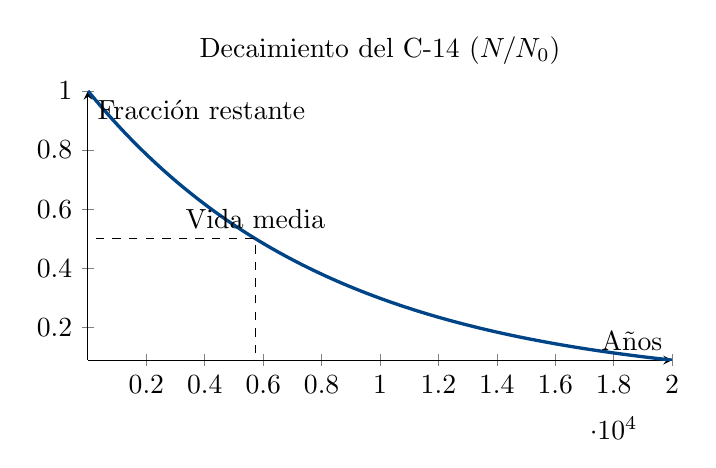
\begin{tikzpicture}
\begin{axis}[width=9cm,height=5cm,xlabel=Años,ylabel={Fracción restante},axis lines=middle,
title={Decaimiento del C-14 ($N/N_0$)}]
\addplot[UANazul,line width=1.2pt,domain=0:20000,samples=80]{0.5^(x/5730)};
\draw[dashed] (axis cs:5730,0) -- (axis cs:5730,0.5) -- (axis cs:0,0.5);
\node[above] at (axis cs:5730,0.5) {Vida media};
\end{axis}
\end{tikzpicture}
\end{center}

\begin{aplbox}{Más aplicaciones de logaritmos y exponenciales}
\textbf{a)} Una inversión de \$8{,}000 gana interés compuesto continuo al 6\% anual. ¿Cuánto vale después de 10 años?\\
\textit{Solución:} $A=8000\,e^{0.06\cdot10}=8000\,e^{0.6}\approx\$14{,}577$.\\[4pt]
\textbf{b)} El nivel sonoro de un concierto es 110 dB. ¿Cuántas veces más intensa es esta onda respecto al umbral de audición $I_0$?\\
\textit{Solución:} $110=10\log(I/I_0)\Rightarrow I/I_0=10^{11}$, es decir, $10^{11}$ veces más intensa.\\[4pt]
\textbf{c)} Un terremoto registra magnitud 7.2 en la escala de Richter y otro magnitud 5.2. ¿Cuántas veces más energía libera el primero?\\
\textit{Solución:} $M=\log(A/A_0)\Rightarrow$ diferencia de 2 unidades implica $A_1/A_2=10^2=100$ veces.
\end{aplbox}

\section{Ejercicios propuestos}

\begin{enumerate}
\item Convierte: $\log_4 64=3$.
\item Convierte: $5^{-2}=1/25$.
\item Calcula: $\log_{27}9$, $\log_84$, $\log0.01$.
\item Expande: $\log_2(x^3/\sqrt y)$.
\item Escribe como un logaritmo: $2\log x-3\log y+\log z$.
\item Resuelve: $\log_4(x+3)=2$.
\item Resuelve: $\log(x-1)+\log(x+2)=1$.
\item Resuelve: $\ln(x+1)-\ln x=\ln3$.
\item Resuelve: $5^{2x+1}=25^{x-1}$.
\item Resuelve: $2^x=13$.
\item Resuelve: $e^{2x}-7e^x+10=0$.
\item pH: calcula pH para $[H^+]=3.5\times10^{-4}$.
\item Una inversión crece al 8\% anual continuo. ¿En cuántos años se duplica?
\item \textit{(Nuevo)} Resuelve (misma base): $\log_6(5x-4)=\log_6(x+8)$.
\item \textit{(Nuevo)} Resuelve (bases diferentes): $\log_4 x=\log_2 9$.
\item \textit{(Nuevo)} Resuelve: $7^{x+2}=3^{x}$ aplicando logaritmo natural.
\item \textit{(Nuevo)} Investiga y explica brevemente por qué Euler usó la letra $e$ para nombrar a la constante $2.71828\ldots$
\item \textbf{(Aplicación)} El número de bacterias en un cultivo se duplica cada 3 horas. Si inicia con 500 bacterias, ¿cuándo alcanzará 32{,}000?
\item \textbf{(Aplicación)} Calcula los decibeles de un sonido cuya intensidad es $10^{-4}$ W/m$^2$, si $I_0=10^{-12}$ W/m$^2$.
\item \textbf{(Aplicación)} Un capital se invierte a interés compuesto continuo al 5\% anual. ¿Cuánto tiempo tarda en triplicarse?
\end{enumerate}

\textbf{Respuestas (1--13):} 1. $4^3=64$\quad 2. $\log_5(1/25)=-2$\quad 3. $2/3;2/3;-2$\quad 4. $3\log_2x-\tfrac12\log_2y$\quad 5. $\log(x^2z/y^3)$\quad 6. $x=13$\quad 7. $x=3$\quad 8. $x=1/2$\quad 9. $x=-3$\quad 10. $x=\log_213\approx3.70$\quad 11. $x=\ln2,\ln5$\quad 12. $\approx3.46$\quad 13. $t=\ln2/0.08\approx8.66$ años.

\textbf{Respuestas (14--20):} 14. $x=3$\quad 15. $\log_29=\dfrac{\ln9}{\ln2}\approx3.17\Rightarrow x=4^{3.17}\approx81$ (equivalente a $x=9^2=81$ por cambio de base directo)\quad 16. $(x+2)\ln7=x\ln3\Rightarrow x=\dfrac{2\ln7}{\ln3-\ln7}\approx-4.59$\quad 17. Euler eligió $e$ posiblemente por ser la primera letra disponible no usada en ese momento, o por relacionarse con ``exponencial''; la introdujo en su obra de 1748 \emph{Introductio in analysin infinitorum}\quad 18. $32000=500\cdot2^{t/3}\Rightarrow t=3\log_264=18$ horas\quad 19. $\beta=10\log(10^{8})=80$ dB\quad 20. $t=\ln3/0.05\approx21.97$ años.

% ============================================================
\begin{thebibliography}{9}
\bibitem{stewart} Stewart, J., Redlin, L., \& Watson, S. (2012). \textit{Precálculo: Matemáticas para el cálculo} (7.\textsuperscript{a} ed.). Cengage Learning.
\bibitem{aufmann} Aufmann, R. N., Barker, V. C., \& Nation, R. D. (2010). \textit{Álgebra y trigonometría} (6.\textsuperscript{a} ed.). Cengage Learning.
\bibitem{larson} Larson, R. (2014). \textit{Precálculo} (9.\textsuperscript{a} ed.). Cengage Learning.
\bibitem{cohen} Cohen, D. (2005). \textit{Precálculo} (5.\textsuperscript{a} ed.). Thomson Learning.
\bibitem{swokowski} Swokowski, E. W., \& Cole, J. A. (2011). \textit{Álgebra y trigonometría con geometría analítica} (13.\textsuperscript{a} ed.). Cengage Learning.
\end{thebibliography}

\end{document}
